\chapter{Setup}
\label{chap:setup}

This chapter is about the first task at hand.
We want to find an archetypal model for the peculiar behavior of the original model.
For this, we first analyze the original model function and note the characteristics.
After that, we construct different models with different characteristics and analyze their behavior as outlined in \Cref{chap:approach}.

\section{Characteristics}
\label{sec:setup.char}

In this section, we will analyze the original model function and note the characteristics.
The first kind of characteristics is the shape of the function.
After that, we will examine the effects that the parameters have on the shape of the function.

\subsection{Function Shape}

\begin{figure}
	\centering
	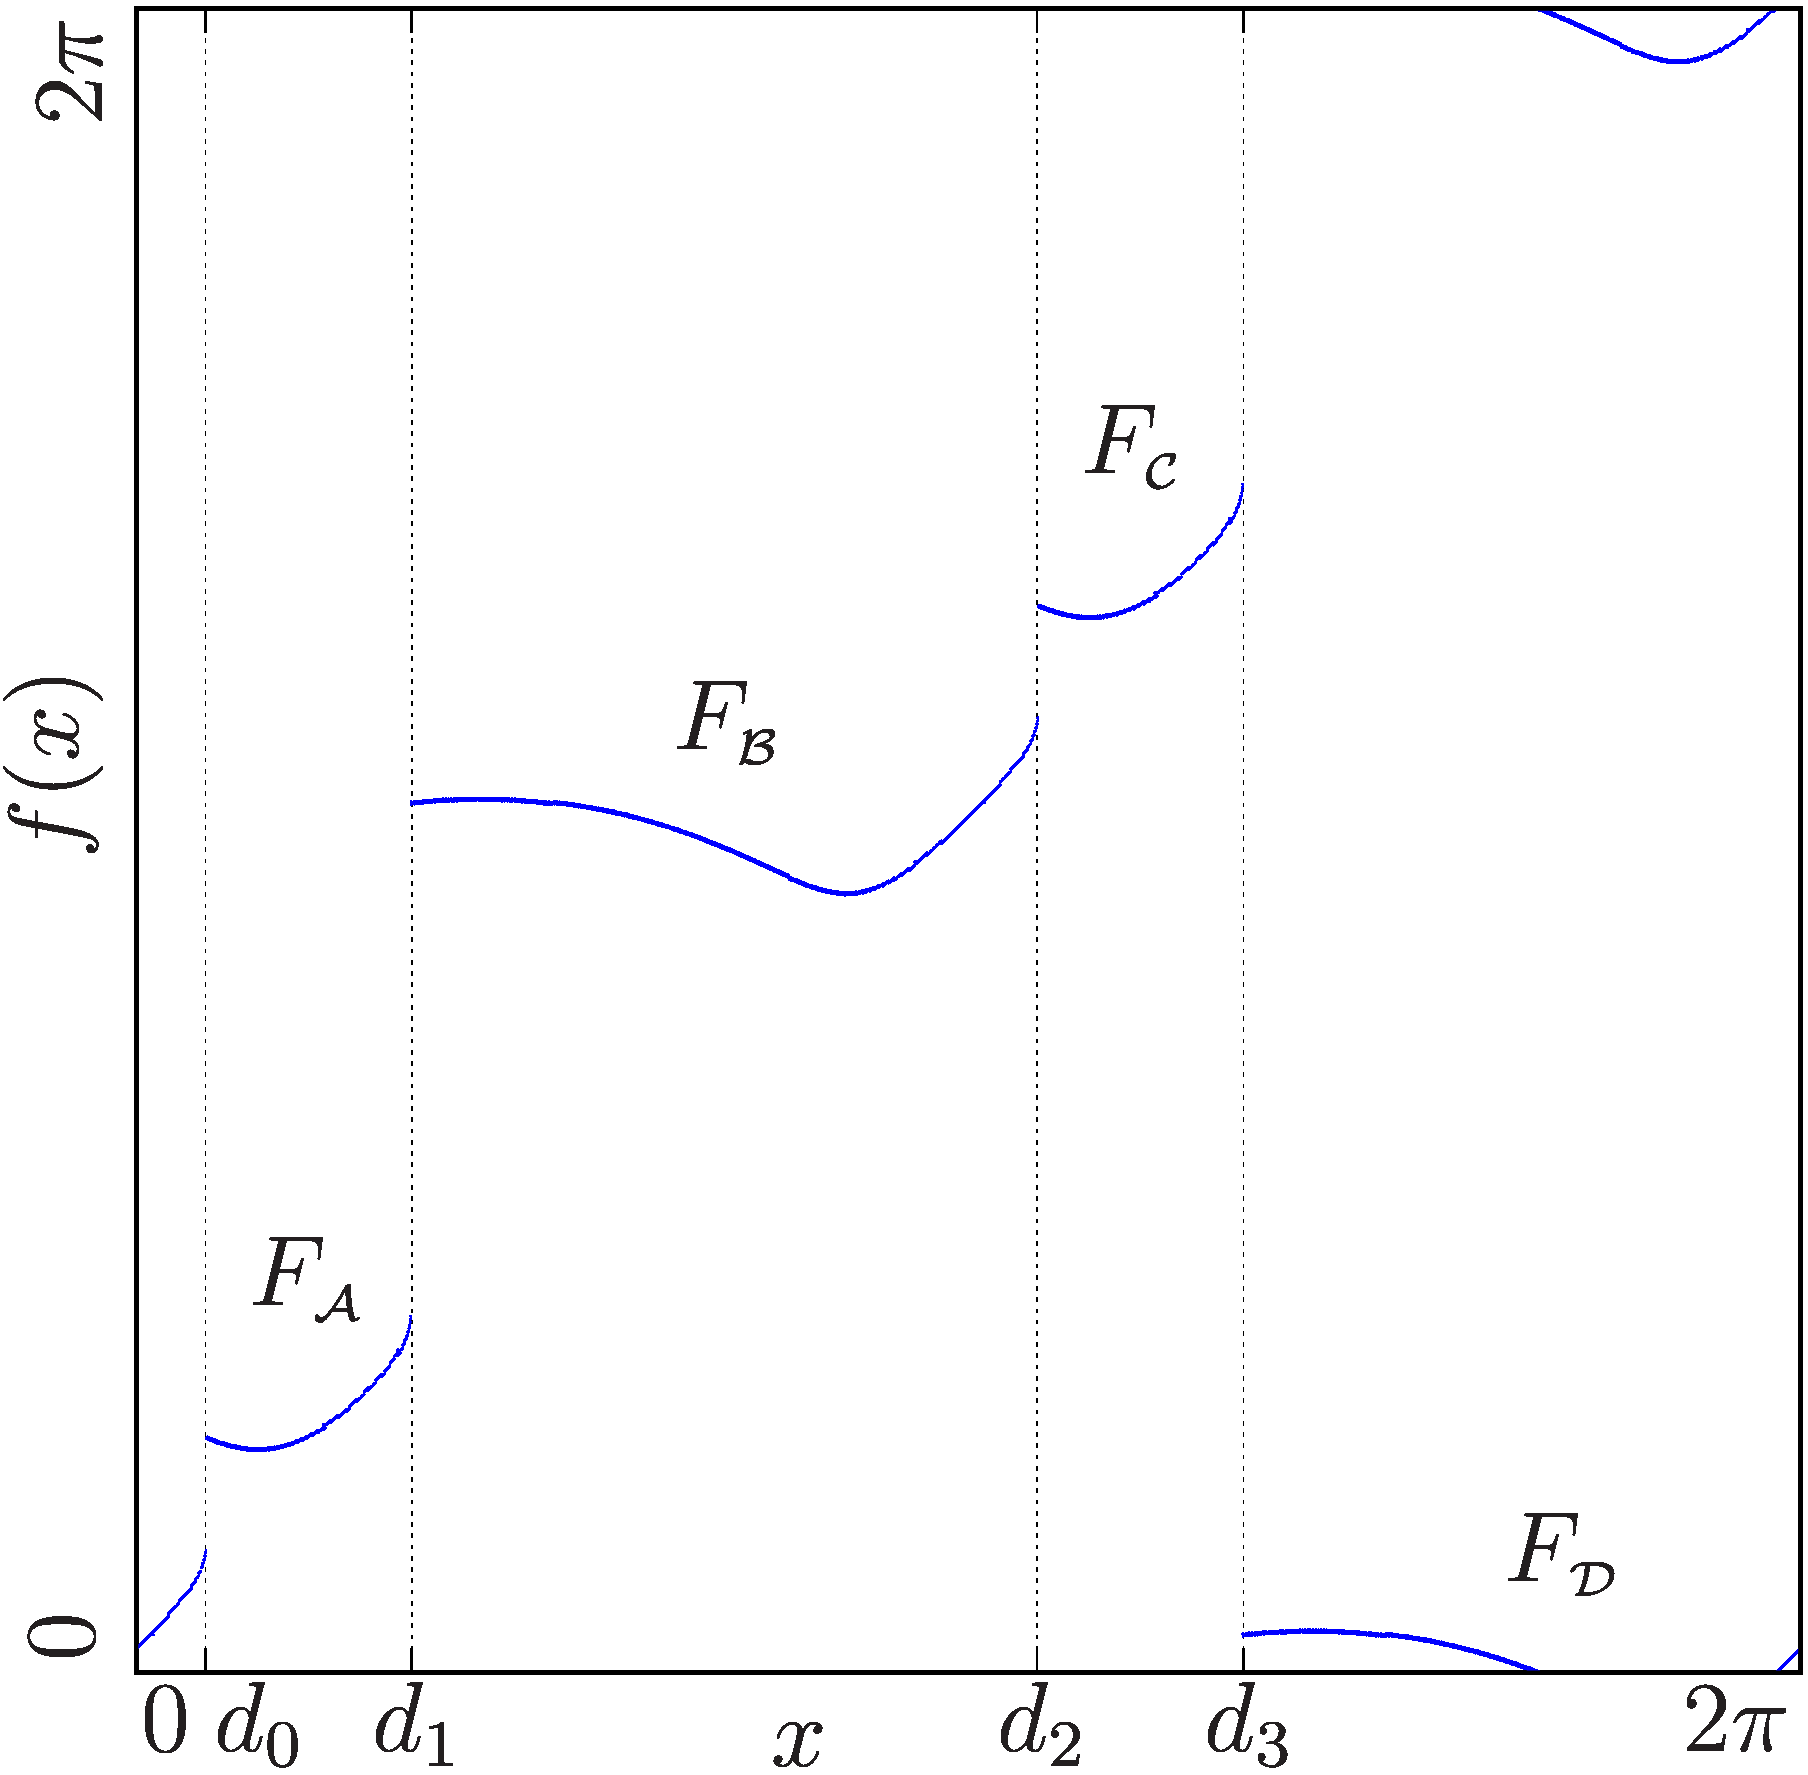
\includegraphics[width=.5 \textwidth]{../Figures/5/5.1/illustration.png}
	\caption[Shape of the original model function]{
		The shape of the original model function at the parameter values $E_0 = 15$ and $\chi_0 = 0.2$.
	}
	\label{fig:setup.char.shape}
\end{figure}

This section is concerned with the overall shape and number of branches of the original model function.

\Cref{fig:setup.char.shape} shows the shape of the original model function.
One can immediately see that the model function has 4 branches.
This is also evident from the model definition given in \Cref{sec:state.og.def}.
Also, we know from \Cref{sec:state.og.dynamics} that the model has the symmetry described by \Cref{equ:state.og.sym}.
So the branches $F_\A$ and $F_\C$ are identical.
The same is true for the branches $F_\B$ and $F_\D$.

There are no fixed points in the parameter regions that this thesis is concerned with.
That means, the function is always larger than the bisector $y=x$.
Also, for the most part the slope of the function is not steep.
Meaning that the absolute value of the model functions derivative is below $1$ for a majority of the state space.
A model where the absolute value of the derivative of its model function is below $1$ for the whole state space is called contractive.
In such a model, every fixed point and cycle is stable.

\subsection{Parameter Effects}
\label{sec:setup.char.paramfx}

This section is concerned with the other types of characteristics, the effects of the parameters of the model on the shape of the model function.
First, it analyzes the combined parameter effects along a chain of parameter regions assocoated with cycles the same period.
After that, it analyzes the isolated effects of the single parameters and decomposes the combined effects into the isolated effects.

\subsection{Combined Effects of Parameters}
\label{sec:setup.char.paramfx.combined}

To replicate the dynamics seen in the model, it is helpful to know, how the model changes along the chains of parameter regions that are associated with cycles of the same period.
This section therefore analyzes the model function at different points in different chains.
\Cref{fig:setup.char.evolution.map} indicates the points used for this analysis.
\Cref{fig:setup.char.evolution.12} shows, how the model function changes along the chain of parameter regions associated with cycles of period 12.
In the figure, there are three functions $F^{A_12}, F^{B_12},$ and $F^{C_12}$.
The function $F^{A_{12}}$ is the model function with the parameters $E_0 = 15.9, \chi_0 = 0.11$.
These parameter values are marked with the point $A_{12}$ in \Cref{fig:setup.char.evolution.map}.
The function $F^{B_{12}}$ is the model function with the parameters $E_0 = 17.07, \chi_0 = 0.182$.
And the function $F^{C_{12}}$ is the model function with the parameters $E_0 = 18.5, \chi_0 = 0.27$.
The parameter values are marked accordingly in \Cref{fig:setup.char.evolution.map}.

\begin{figure}
	\centering
	\subfloat[Points]{
		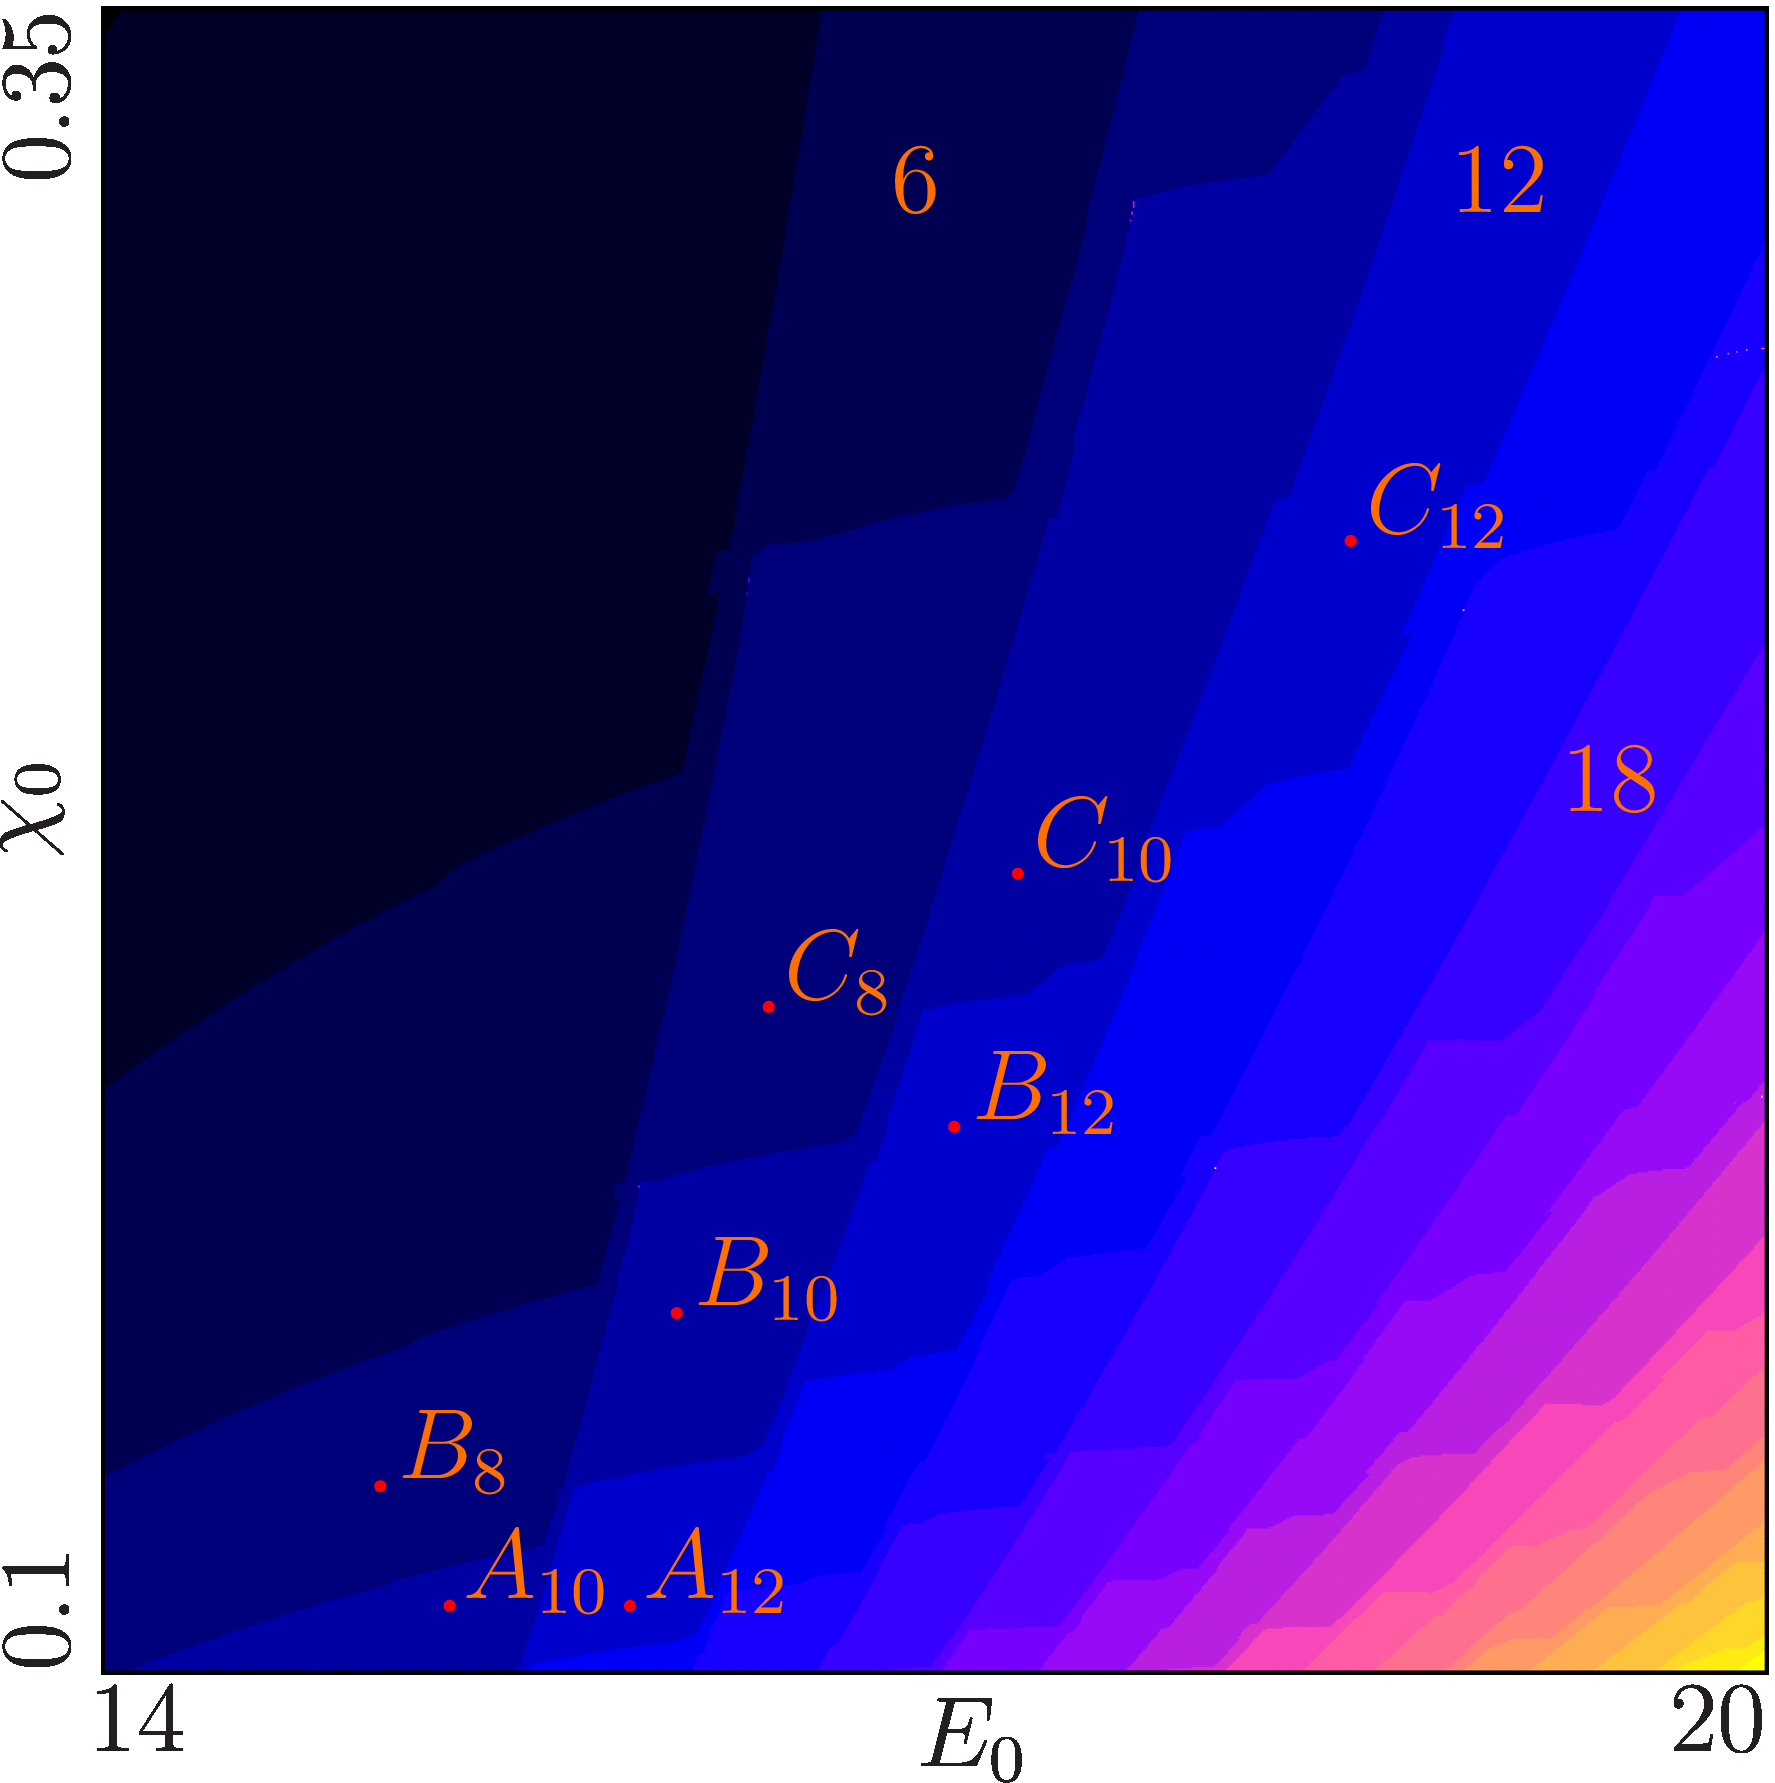
\includegraphics[width=.4 \textwidth]{../Figures/5/5.2a/result.png}
		\label{fig:setup.char.evolution.map}
	}
	\subfloat[Period $12$]{
		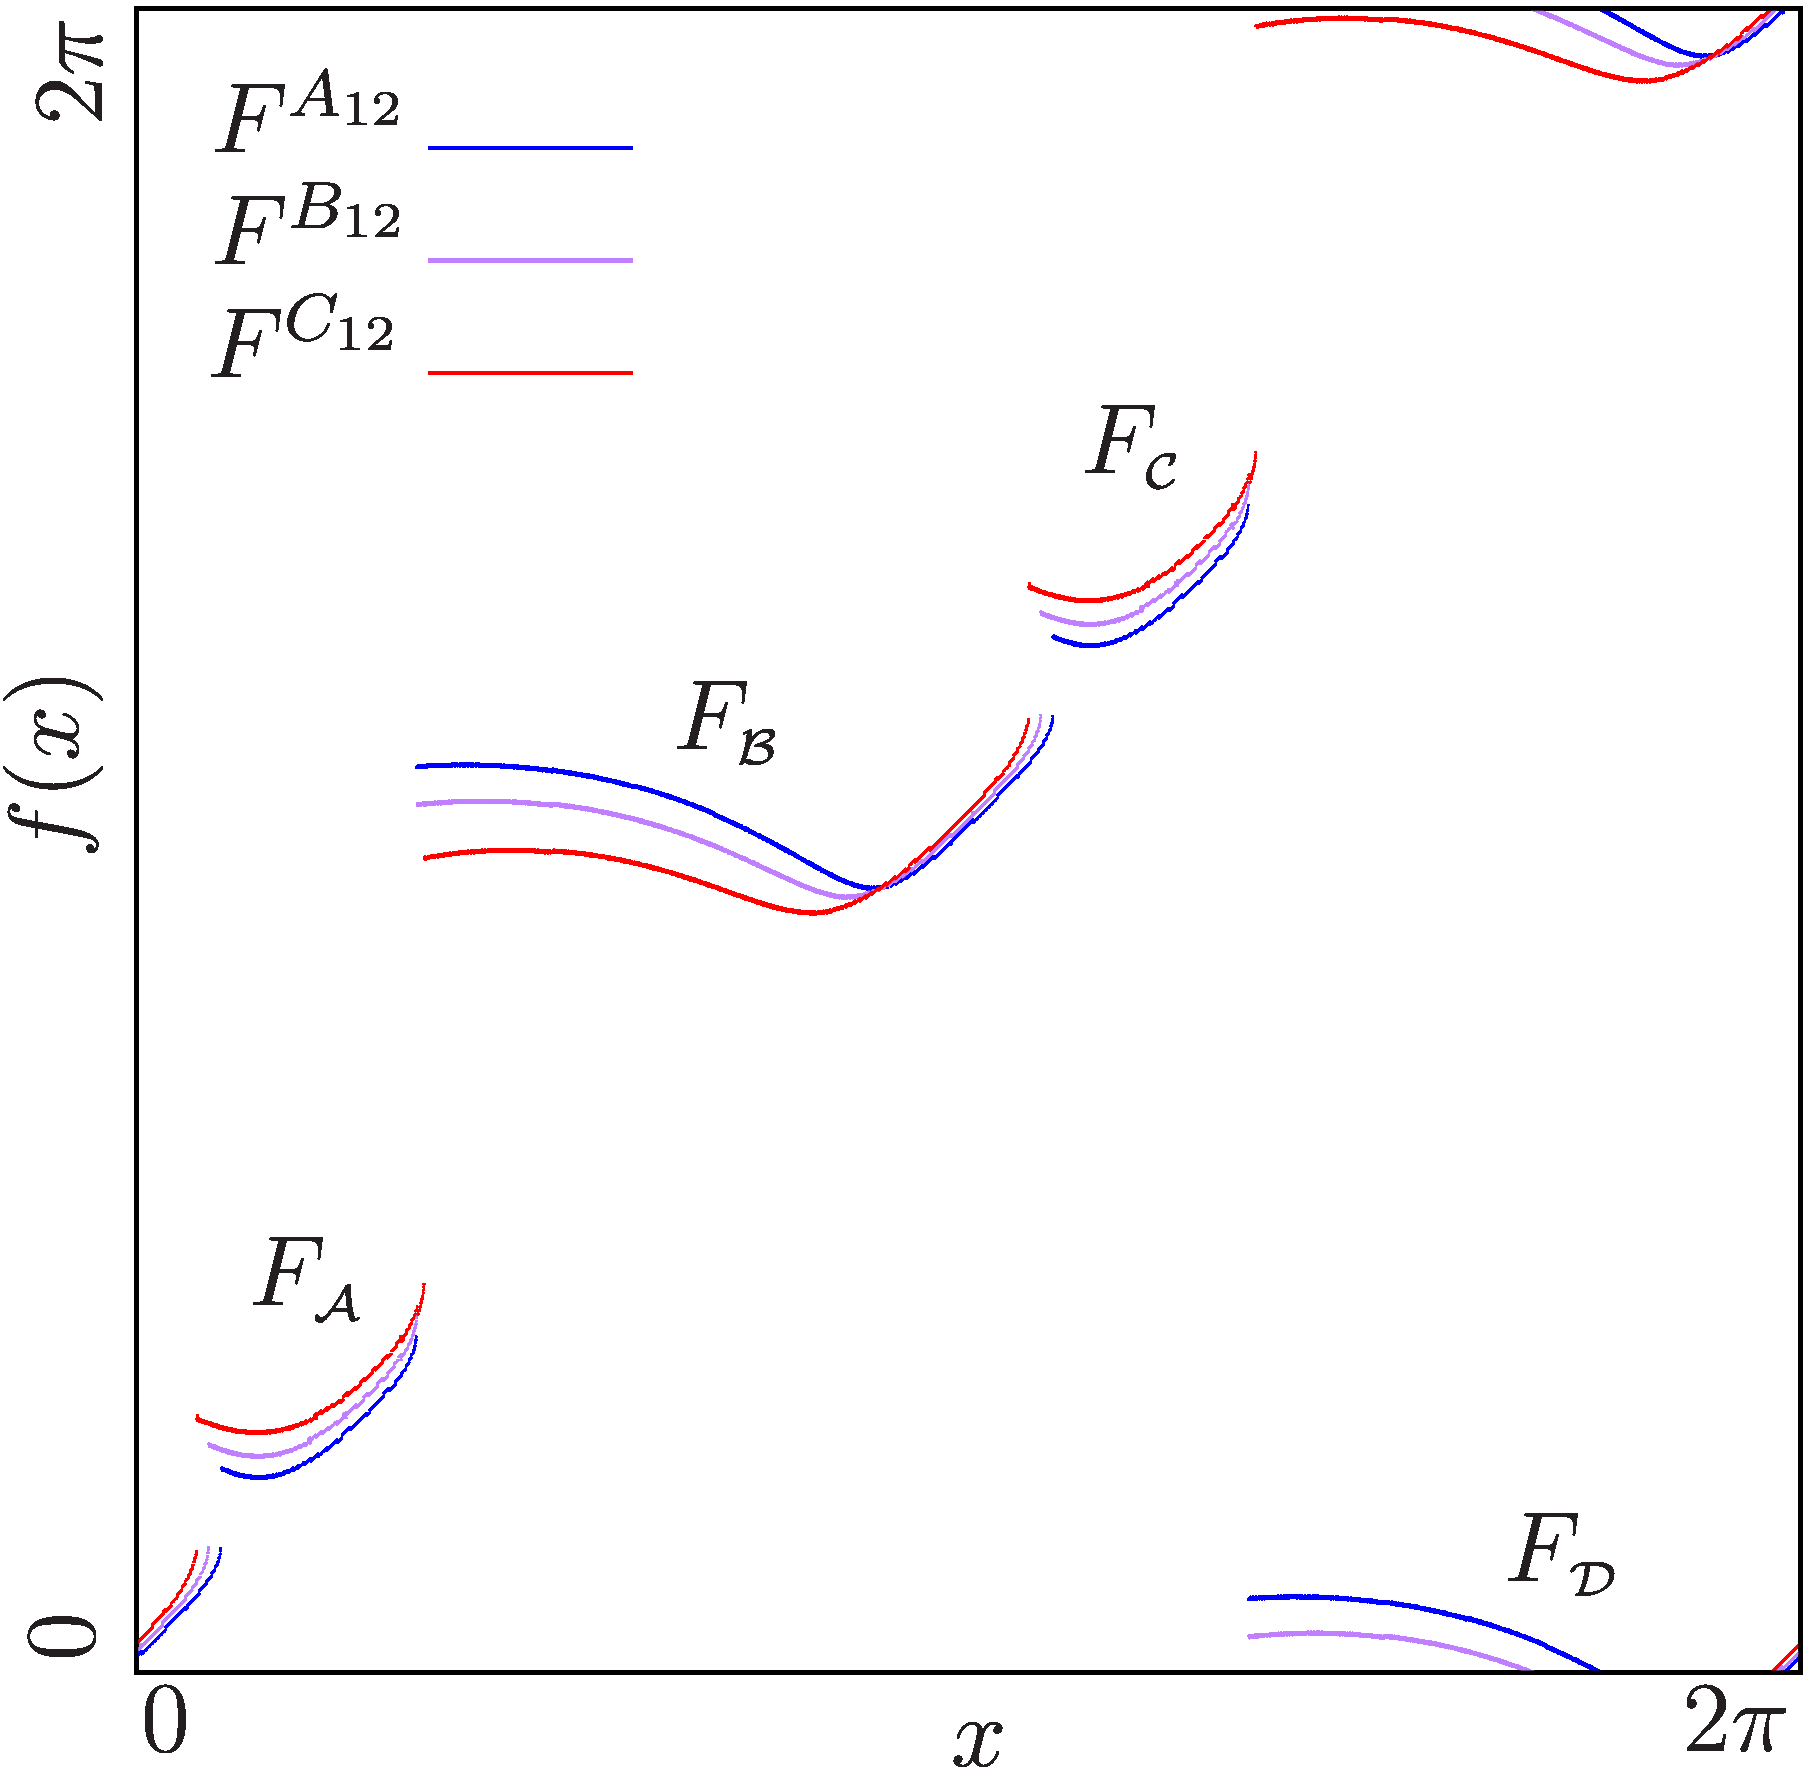
\includegraphics[width=.4 \textwidth]{../Figures/5/5.2b/illustration.png}
		\label{fig:setup.char.evolution.12}
	} \\
	\subfloat[Period $10$]{
		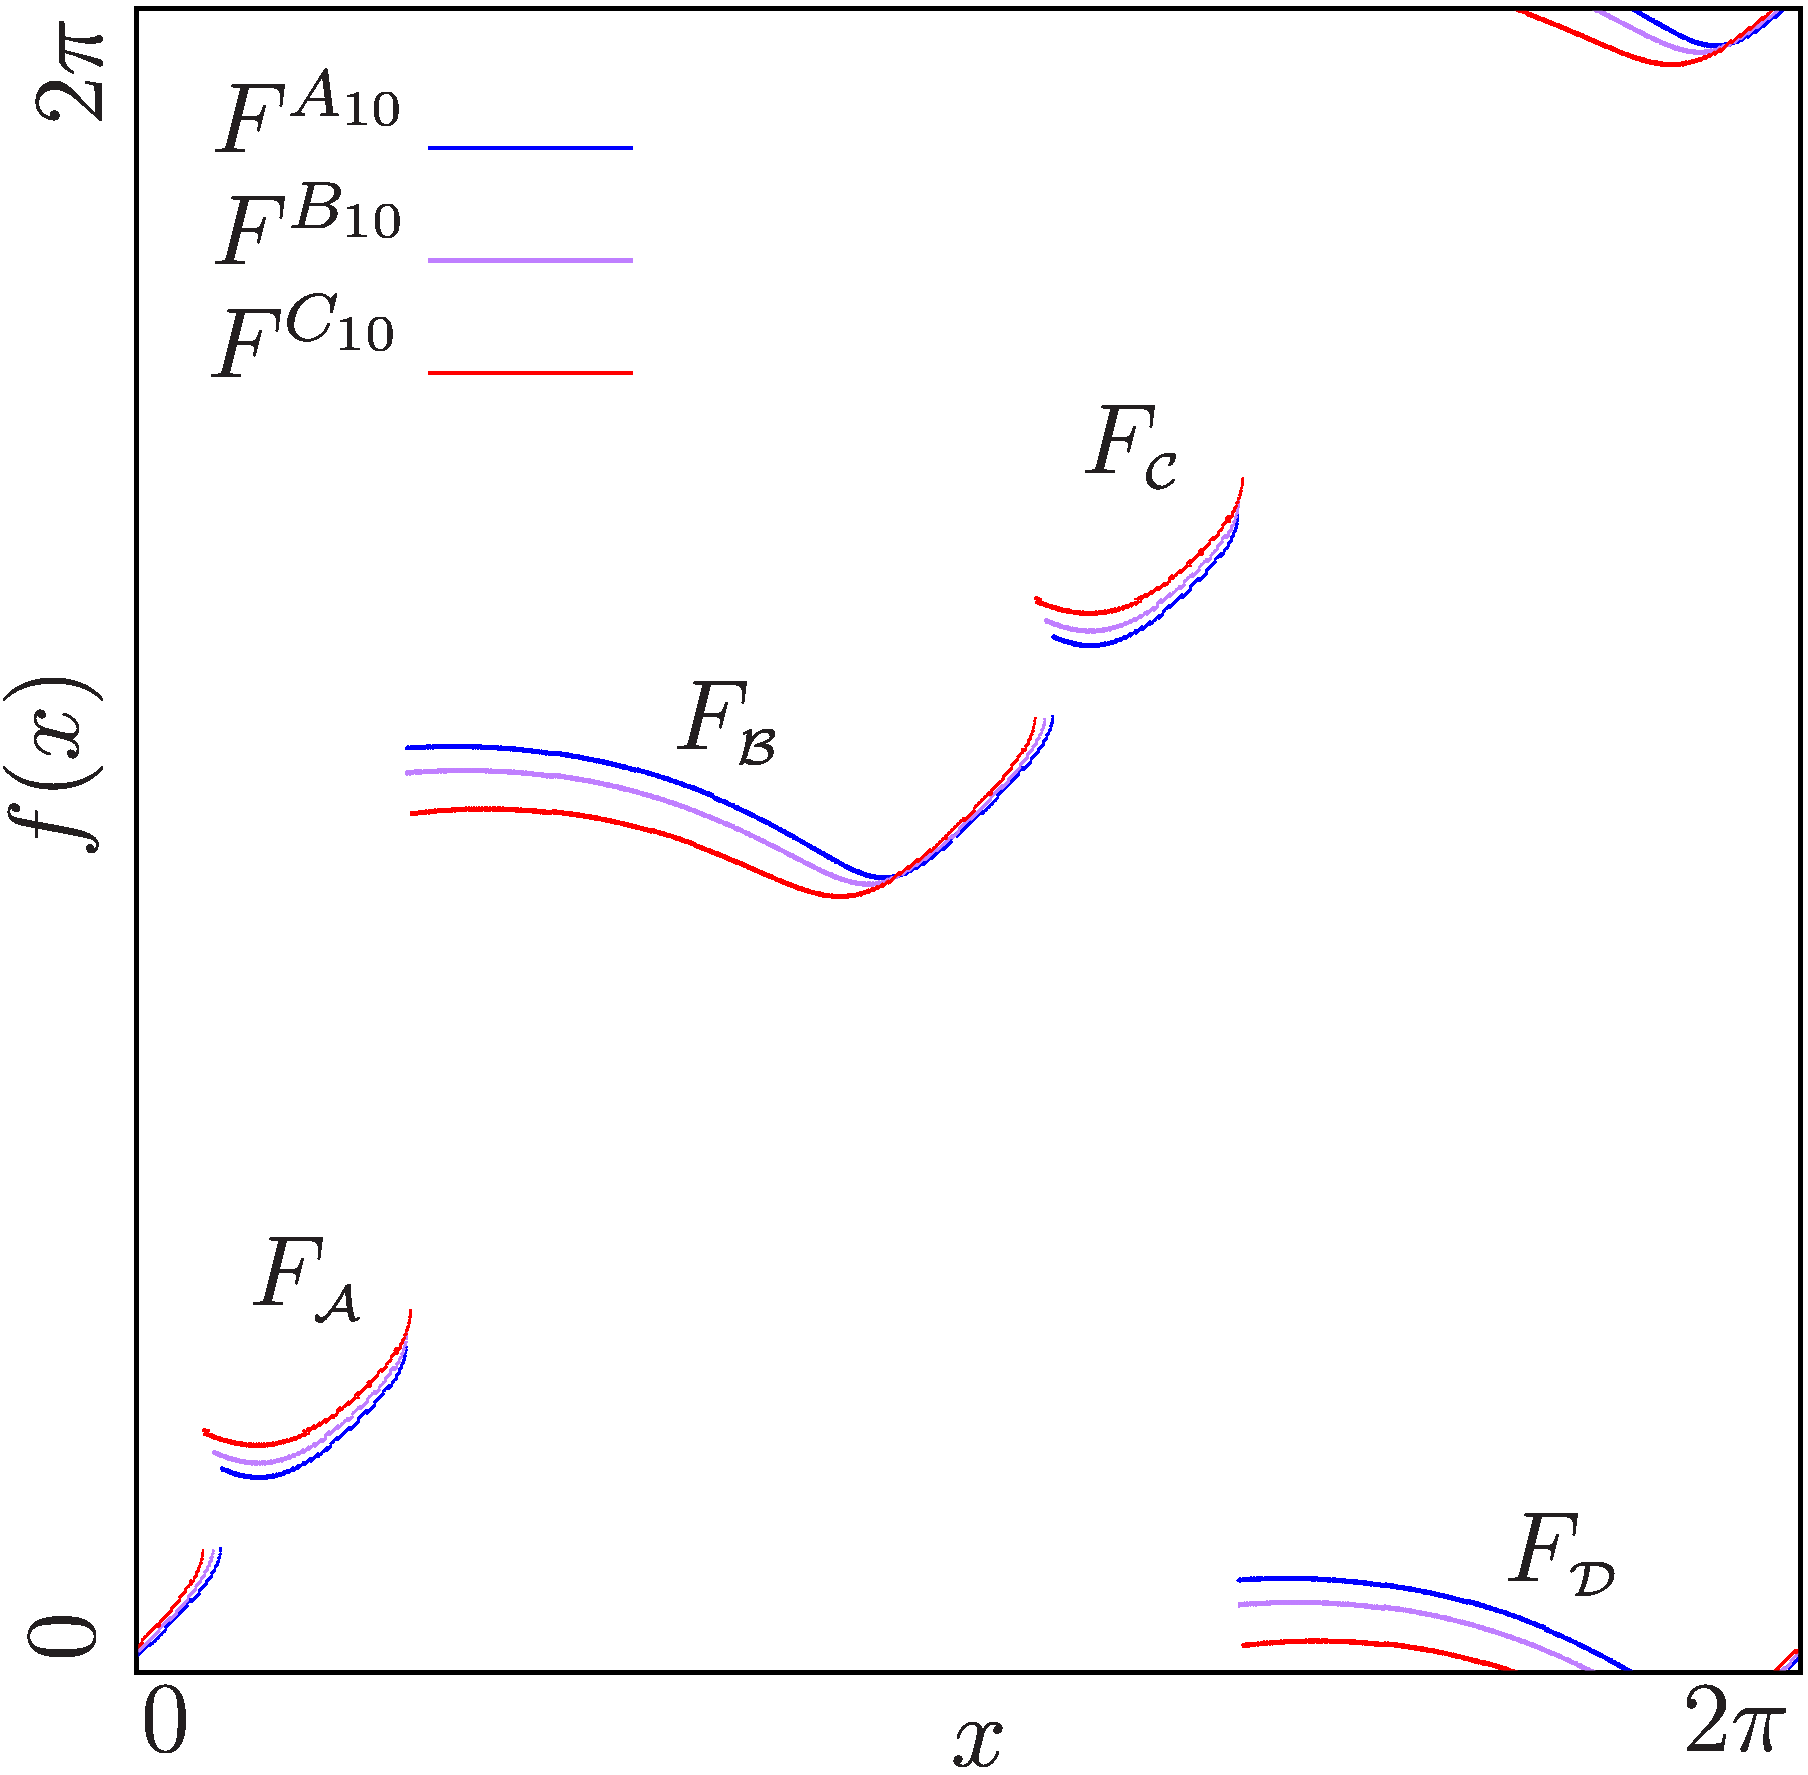
\includegraphics[width=.4 \textwidth]{../Figures/5/5.2c/illustration.png}
		\label{fig:setup.char.evolution.10}
	}
	\subfloat[Period $8$]{
		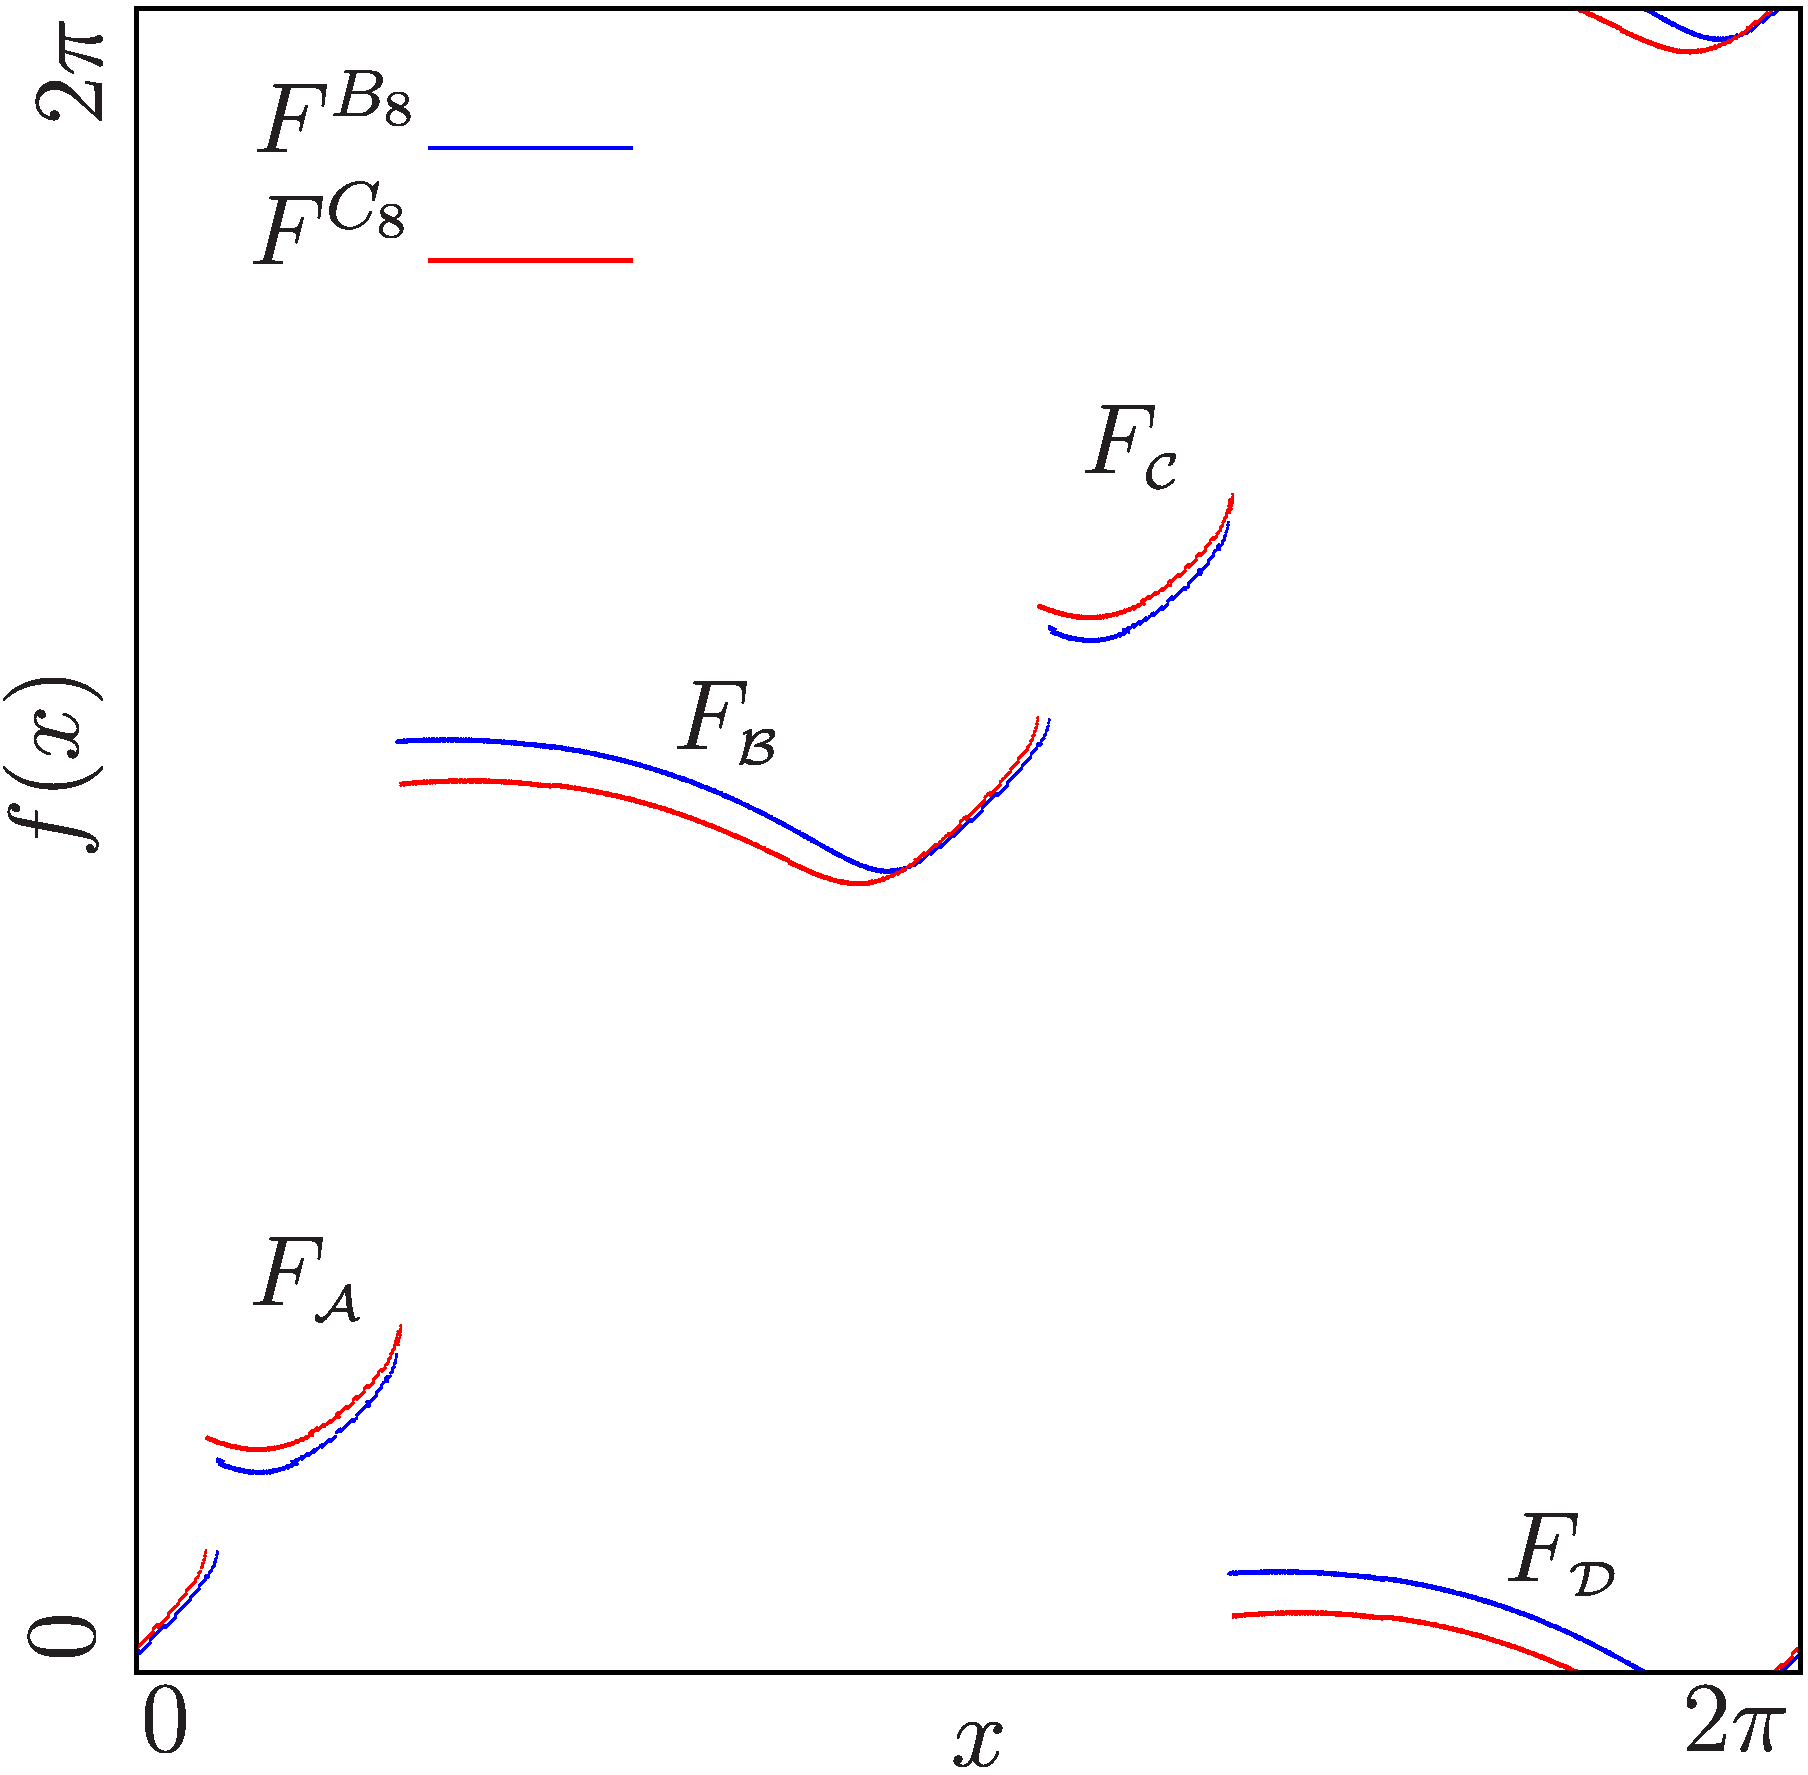
\includegraphics[width=.4 \textwidth]{../Figures/5/5.2d/illustration.png}
		\label{fig:setup.char.evolution.08}
	}
	\caption[The effects of the parameters on the original model function]{
		The effects of the parameters on the original model function illustrated by plotting the model function at different parameter values.
		The parameters $\beta = 1, f = 150, L = 4.2 \cdot 10^{-3}, R = 2, V_m = 5,$ and $\mu = 0.5$ are fixed.
		(a) shows a 2D scan of the periods associated with parameter regions in the original model.
		The parameters $E_0$ and $\chi_0$ are varied in the ranges $[14, 20]$ and $[0.1, 0.35]$.
		The points in this scan mark the parameter values used for plotting the model function in (b), (c), and (d).
		(b) shows the evolution of the shape of the model function along the chain of parameter regions associated with the period 12.
		The function $F^{A_{12}}$ is the model function with the parameter values at the point $A_{12}$ where $E_0 = 15.9$ and $\chi_0 = 0.11$,
		$F^{B_{12}}$ at the point $B_{12}$ where $E_0 = 17.07$ and $\chi_0 = 0.182$,
		and $F^{C_{12}}$ at the point $C_{12}$ where $E_0 = 18.5$ and $\chi_0 = 0.27$.
		(c) shows the evolution of the shape of the model function along the chain of parameter regions associated with the period 10.
		Here, $F^{A_{10}}$ is the model function with the parameters at the point $A_{10}$ where $E_0 = 15.25$ and $\chi_0 = 0.11$,
		$F^{B_{10}}$ at the point $B_{10}$ where $E_0 = 16.07$ and $\chi_0 = 0.154$,
		and $F^{C_{10}}$ at the point $C_{10}$ where $E_0 = 17.3$ and $\chi_0 = 0.22$.
		And (d) shows the evolution of the shape of the model function along the chain of parameter regions associated with the period 8.
		Here, $F^{B_8}$ is the model function with the parameter values at the point $B_8$ where $E_0 = 15$ and $\chi_0 = 0.128$,
		and $F^{C_8}$ at the point $C_8$ where $E_0 = 16.4$ and $\chi_0 = 0.2$.
	}
	\label{fig:setup.char.evolution.combined}
\end{figure}

The most notable changes are the following.
\begin{enumerate}
	\item The values of the whole branches $F_\A$ and $F_\C$ get larger.
	      This change is most notable at the left borders of the branches.
	      The values on the left sides of the branches are affected more by this change than the values on the right sides.
	\item The values on the left sides of the branches $F_\B$ and $F_\D$ get smaller while the values on the right sides are not affected much.
	\item The local minima of the branches $F_\B$ and $F_\D$ move to the left, and their values get smaller.
\end{enumerate}
One smaller change is that the border between branches $F_\B$ and $F_\C$ moves left.
Note that the same change happens to the border between the branches $F_\D$ and $F_\A$ due to the symmetry of the function.

The same effects can be observed in the chains of parameter regions associated with cycles of periods $10$ and $8$, respectively.
For the chain of parameter regions associated with cycles of period $10$, the model function is plotted in \Cref{fig:setup.char.evolution.10} at the three points $A_{10}, B_{10},$ and $C_{10}$ marked in \Cref{fig:setup.char.evolution.map}.
Again, the values of the whole branches $F_\A$ and $F_\C$ are larger in $F^{C_{10}}$ than they are in $F^{A_{10}}$.
And the values on the left sides of the branches $F_\B$ and $F_\D$ are smaller in $F^{C_{10}}$ than they are in $F^{A_{10}}$.
Also, the local minima on those branches move left and down.
For the chain of parameter regions associated with cycles of period $8$, the model function is plotted in \Cref{fig:setup.char.evolution.08} at the two points $B_8$ and $C_8$ marked in \Cref{fig:setup.char.evolution.map}.
And the values of the branches undergo the same changes again from the model function $F^{B_8}$ to $F^{C_8}$.

\subsection{Individual Effects of Parameters}
\label{sec:setup.char.paramfx.individual}

The effects of the parameters described above, always include a change in both parameters $E_0$ and $\chi_0$.
To reproduce the bifurcation structures, it is important to know which effects on the function each parameter has individually.
This section focuses on the isolated effects of each parameter by fixing one of the parameters and only varying the other one and observing the effects of this parameter on the shape of the model function.

\begin{figure}
	\centering
	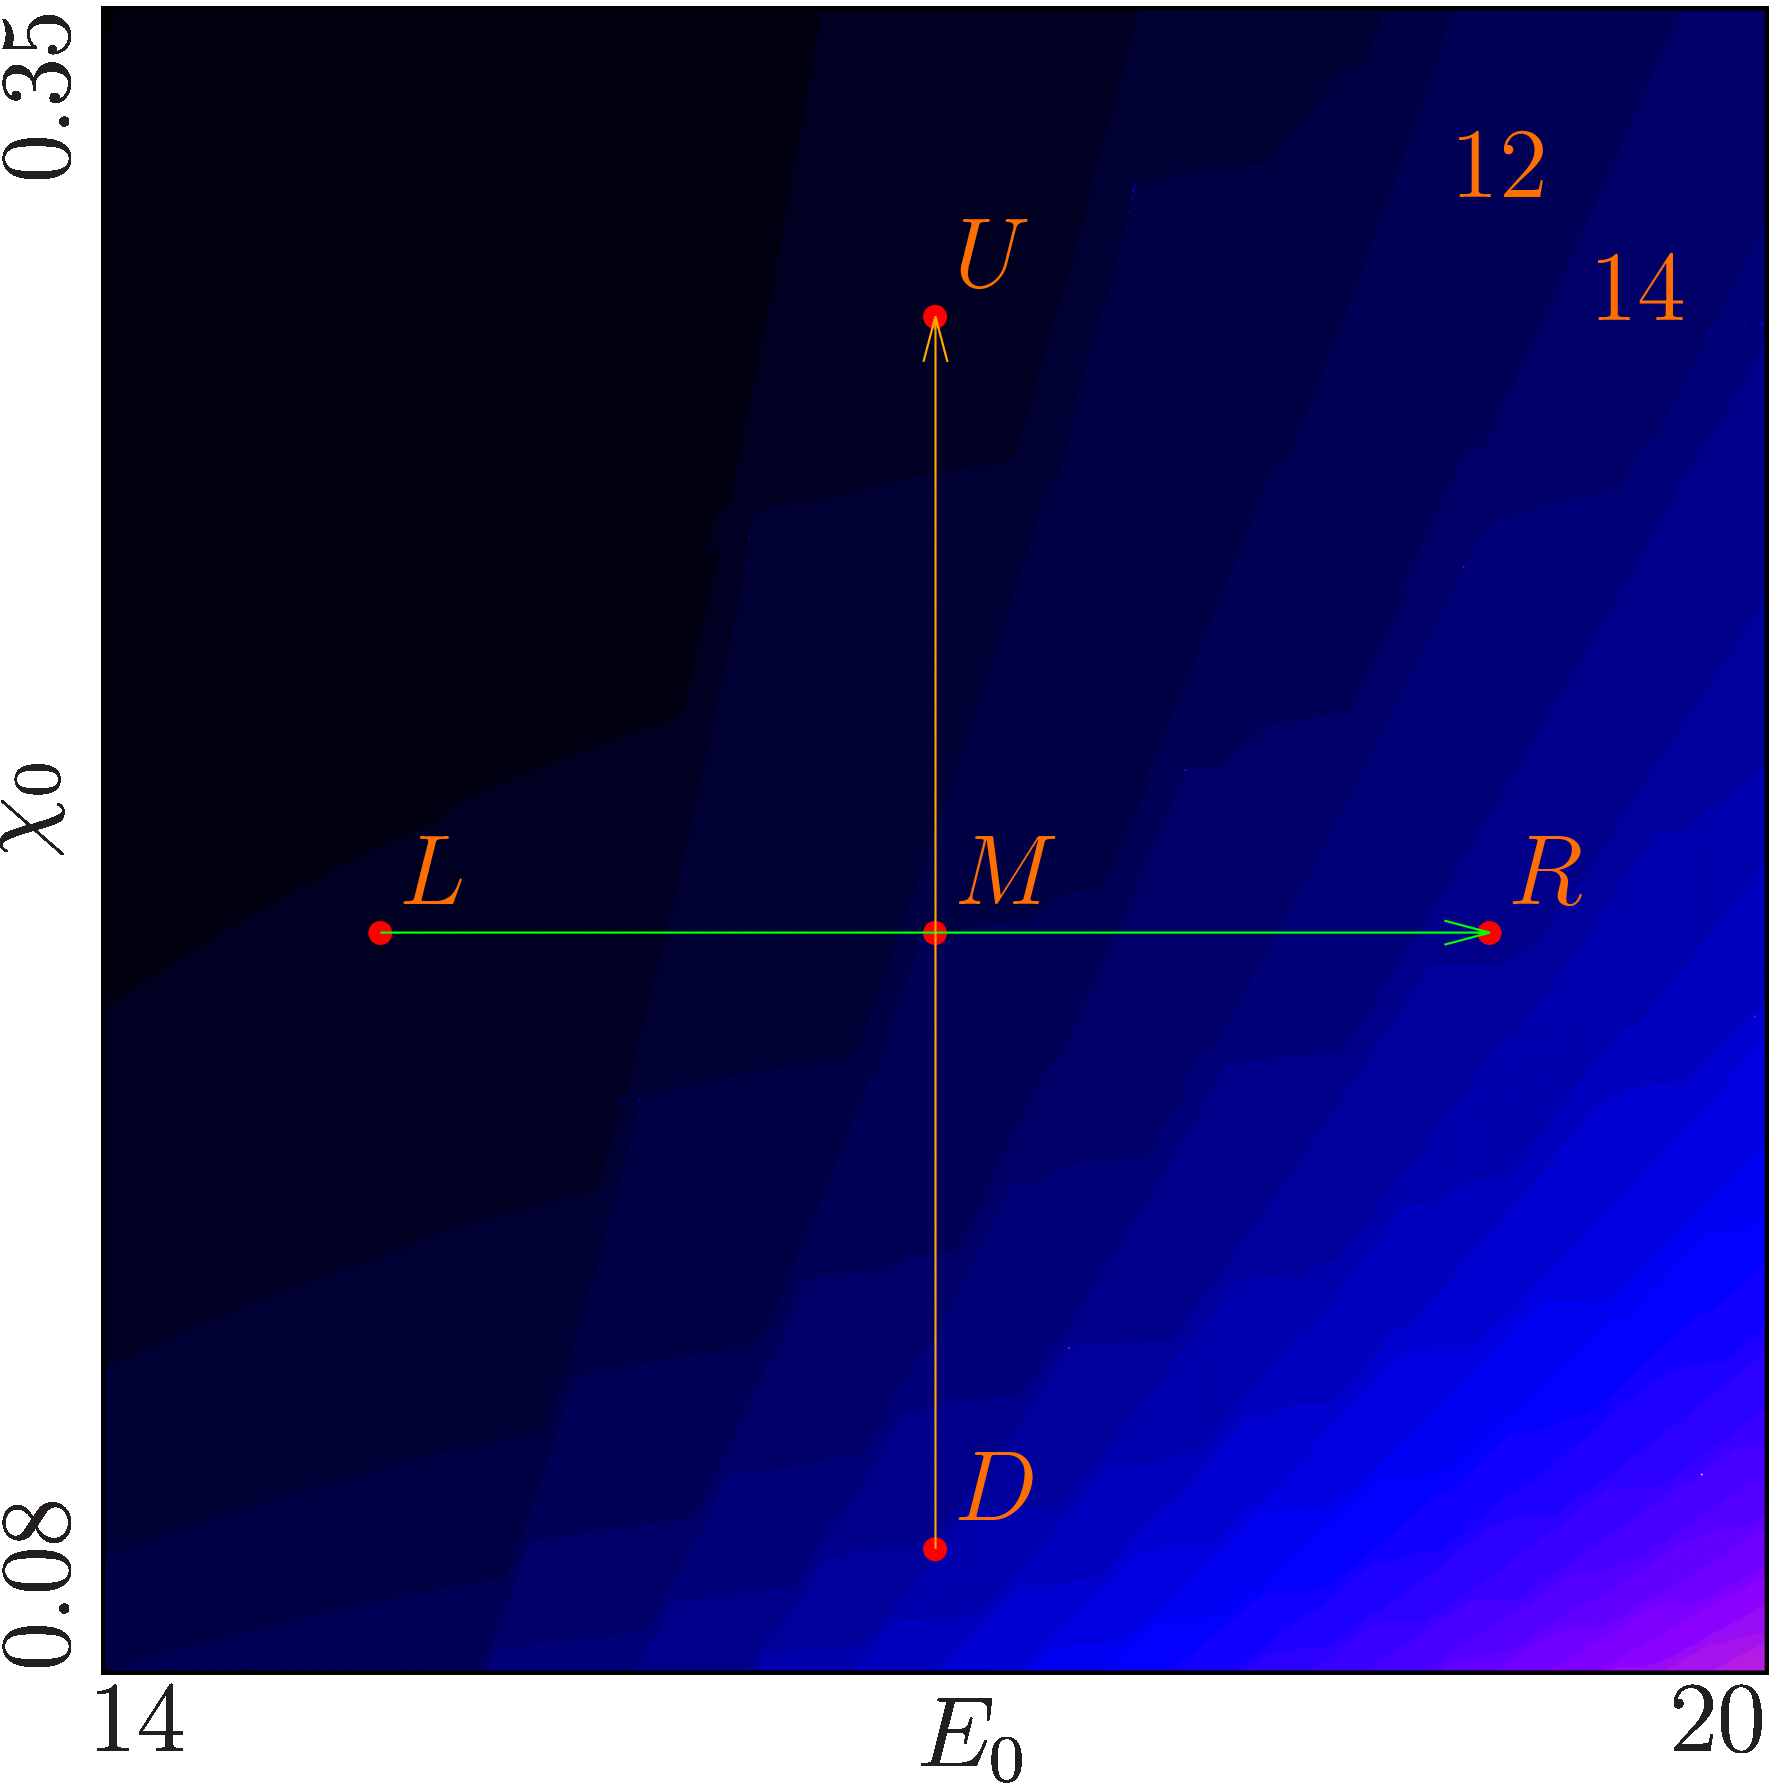
\includegraphics[width=0.4\textwidth]{../Figures/5/5.3/result.png}
	\caption[The parameter ranges examined to analyze the isolated effects of parameters on the original model function]{
		2D scan of the periods associated with parameter regions in the original model.
		The parameters $\beta = 1, f = 150, L = 4.2 \cdot 10^{-3}, R = 2, V_m = 5,$ and $\mu = 0.5$ are fixed.
		The parameters $E_0$ and $\chi_0$ are varied in the ranges $[14, 20]$ and $[0.08, 0.35]$.
		It illustrates the parameter ranges used to analyze the isolated effects of the parameters $E_0$ and $\chi_0$ on the original model function.
		The green arrow indicates the parameter range used to analyze the effects of the parameter $E_0$, while the orange arrow indicates the parameter range used to analyze the effects of the parameter $\chi_0$ on the original model function.
		The points $L, M, R, D,$ and $U$ mark the parameter values used for the cobweb diagrams in \Cref{fig:setup.char.evolution.single}.
	}
	\label{fig:setup.char.evolution.single.map}
\end{figure}

For the effects of the parameter $E_0$, $\chi_0 = 0.2$ is fixed and $E_0$ is varied in the parameter range $[15, 19]$.
This is marked as the green arrow in \Cref{fig:setup.char.evolution.single.map}.
As before, the model function is plotted at three parameter values in one figure.
The functions are visualized in \Cref{fig:setup.char.evolution.e0}.
$F^L$ is the model function with $E_0 = 15$, $F^M$ is the model function with $E_0 = 17$, and $F^R$ is the model function with $E_0 = 17$.
$\chi_0 = 0.2$ is the same for all functions $F^L, F^M,$ and $F^R$.
The parameter values are marked with the points $L, M,$ and $R$ in \Cref{fig:setup.char.evolution.single.map}.
One can see that they are all on the green arrow mentioned before.
The following changes can be observed.
\begin{enumerate}
	\item The values on the left sides of the branches $F_\B$ and $F_\D$ get smaller while the values on the right sides are not affected much.	\item The local minima of the branches $F_\B$ and $F_\D$ move left, and their values get smaller.
	\item The border between the branches $F_\A$ and $F_\B$ moves to the right.
	      The same is true for the border between the branches $F_\C$ and $F_\D$ because of the symmetry in the original model.
	\item The values at the right borders of branches $F_\A$ and $F_\C$ get larger. This is caused by the border between branches $F_\A$ and $F_B$ moving to the right.
\end{enumerate}

For the effects of the parameter $\chi_0$, $E_0 = 17$ is fixed and $\chi_0$ is varied in the parameter range $[0.125, 0.3]$.
This parameter range is marked with an orange arrow in \Cref{fig:setup.char.evolution.single.map}.
Again, the model function is plotted at three parameter values in one figure.
The functions are visualized in \Cref{fig:setup.char.evolution.hi}.
$F^D$ is the model function with $\chi_0 = 0.1$, $F^M$ is the model function with $\chi_0 = 0.2$, and $F^U$ is the model function with $\chi_0 = 0.3$.
$E_0 = 15$ is the same for all functions $F^D, F^M,$ and $F^U$.
The parameter values are marked with the points $D, M,$ and $U$ in \Cref{fig:setup.char.evolution.single.map}.
One can see that they are all on the orange arrow mentioned before.
The following pronounced changes can be observed.
\begin{enumerate}
	\item The values of the whole branches $F_\A$ and $F_\C$ get larger.
	\item The border between the branches $F_\A$ and $F_\B$ moves to the left.
	      The same is true for the border between the branches $F_\C$ and $F_\D$.
\end{enumerate}
Two other smaller changes that can be observed are the following.
\begin{enumerate}
	\item The values on the right sides of the branches $F_\B$ and $F_\D$ get larger.
	      This includes the values of the local minima on these branches.
	\item The border between the branches $F_\B$ and $F_\C$ moves to the left.
	      The same is true for the border between the branches $F_\D$ and $F_\A$.
\end{enumerate}

\begin{figure}
	\centering
	\subfloat[$E_0$]{
		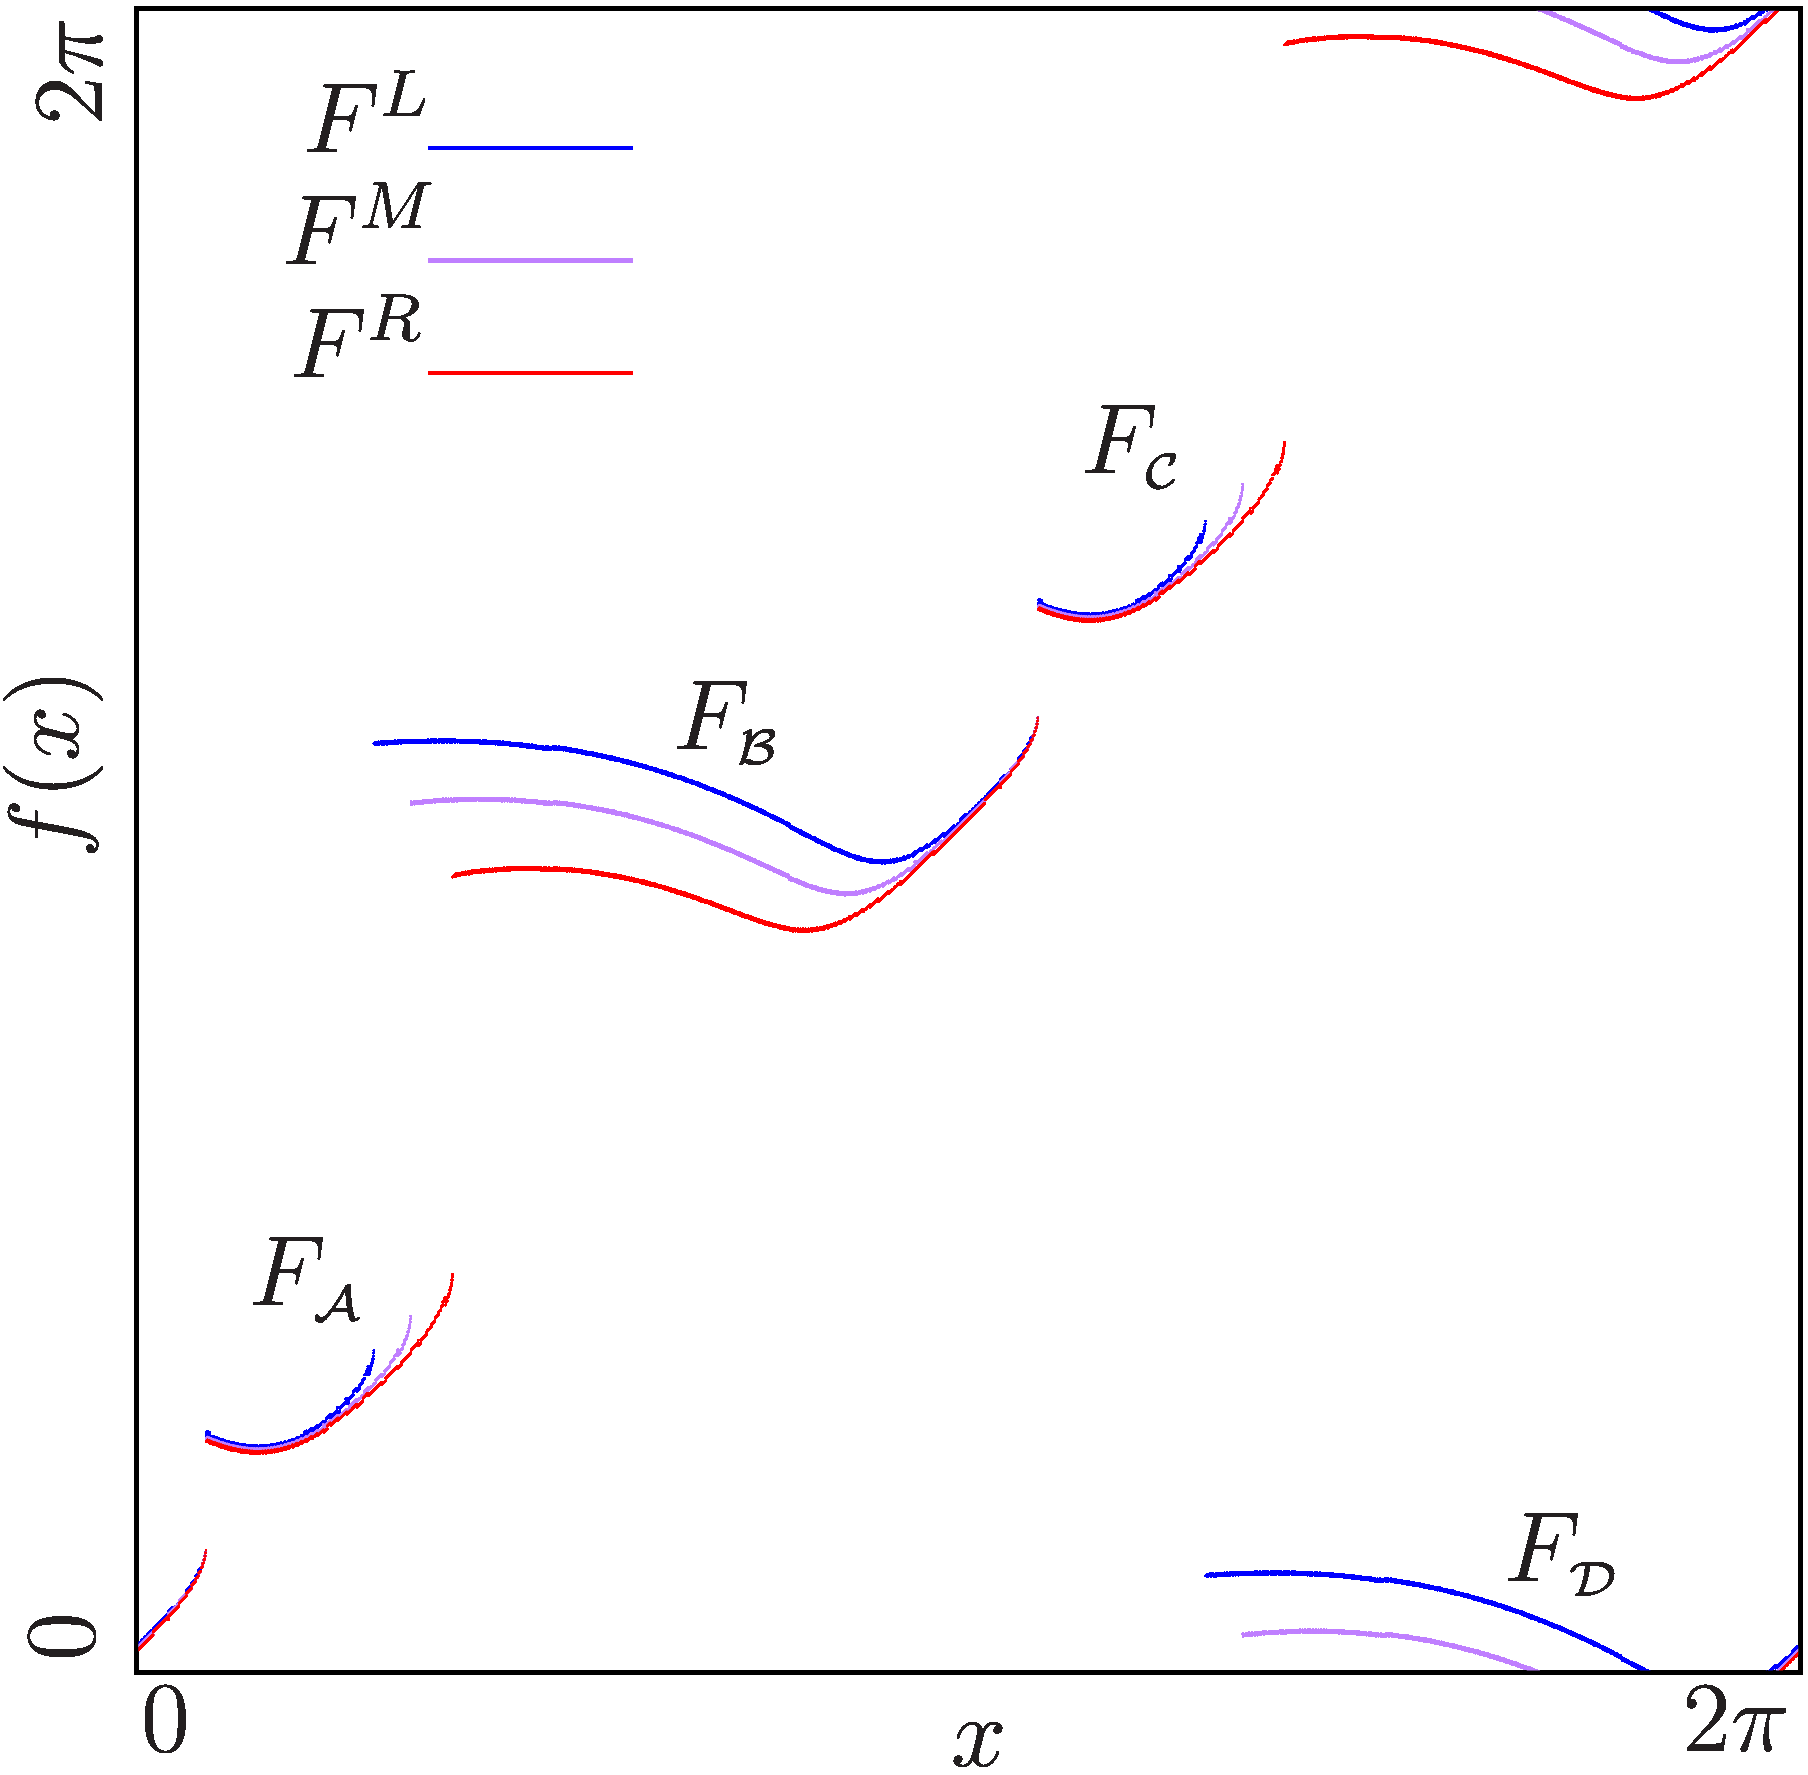
\includegraphics[width=.4 \textwidth]{../Figures/5/5.4a/illustration.png}
		\label{fig:setup.char.evolution.e0}
	}
	\subfloat[$\chi_0$]{
		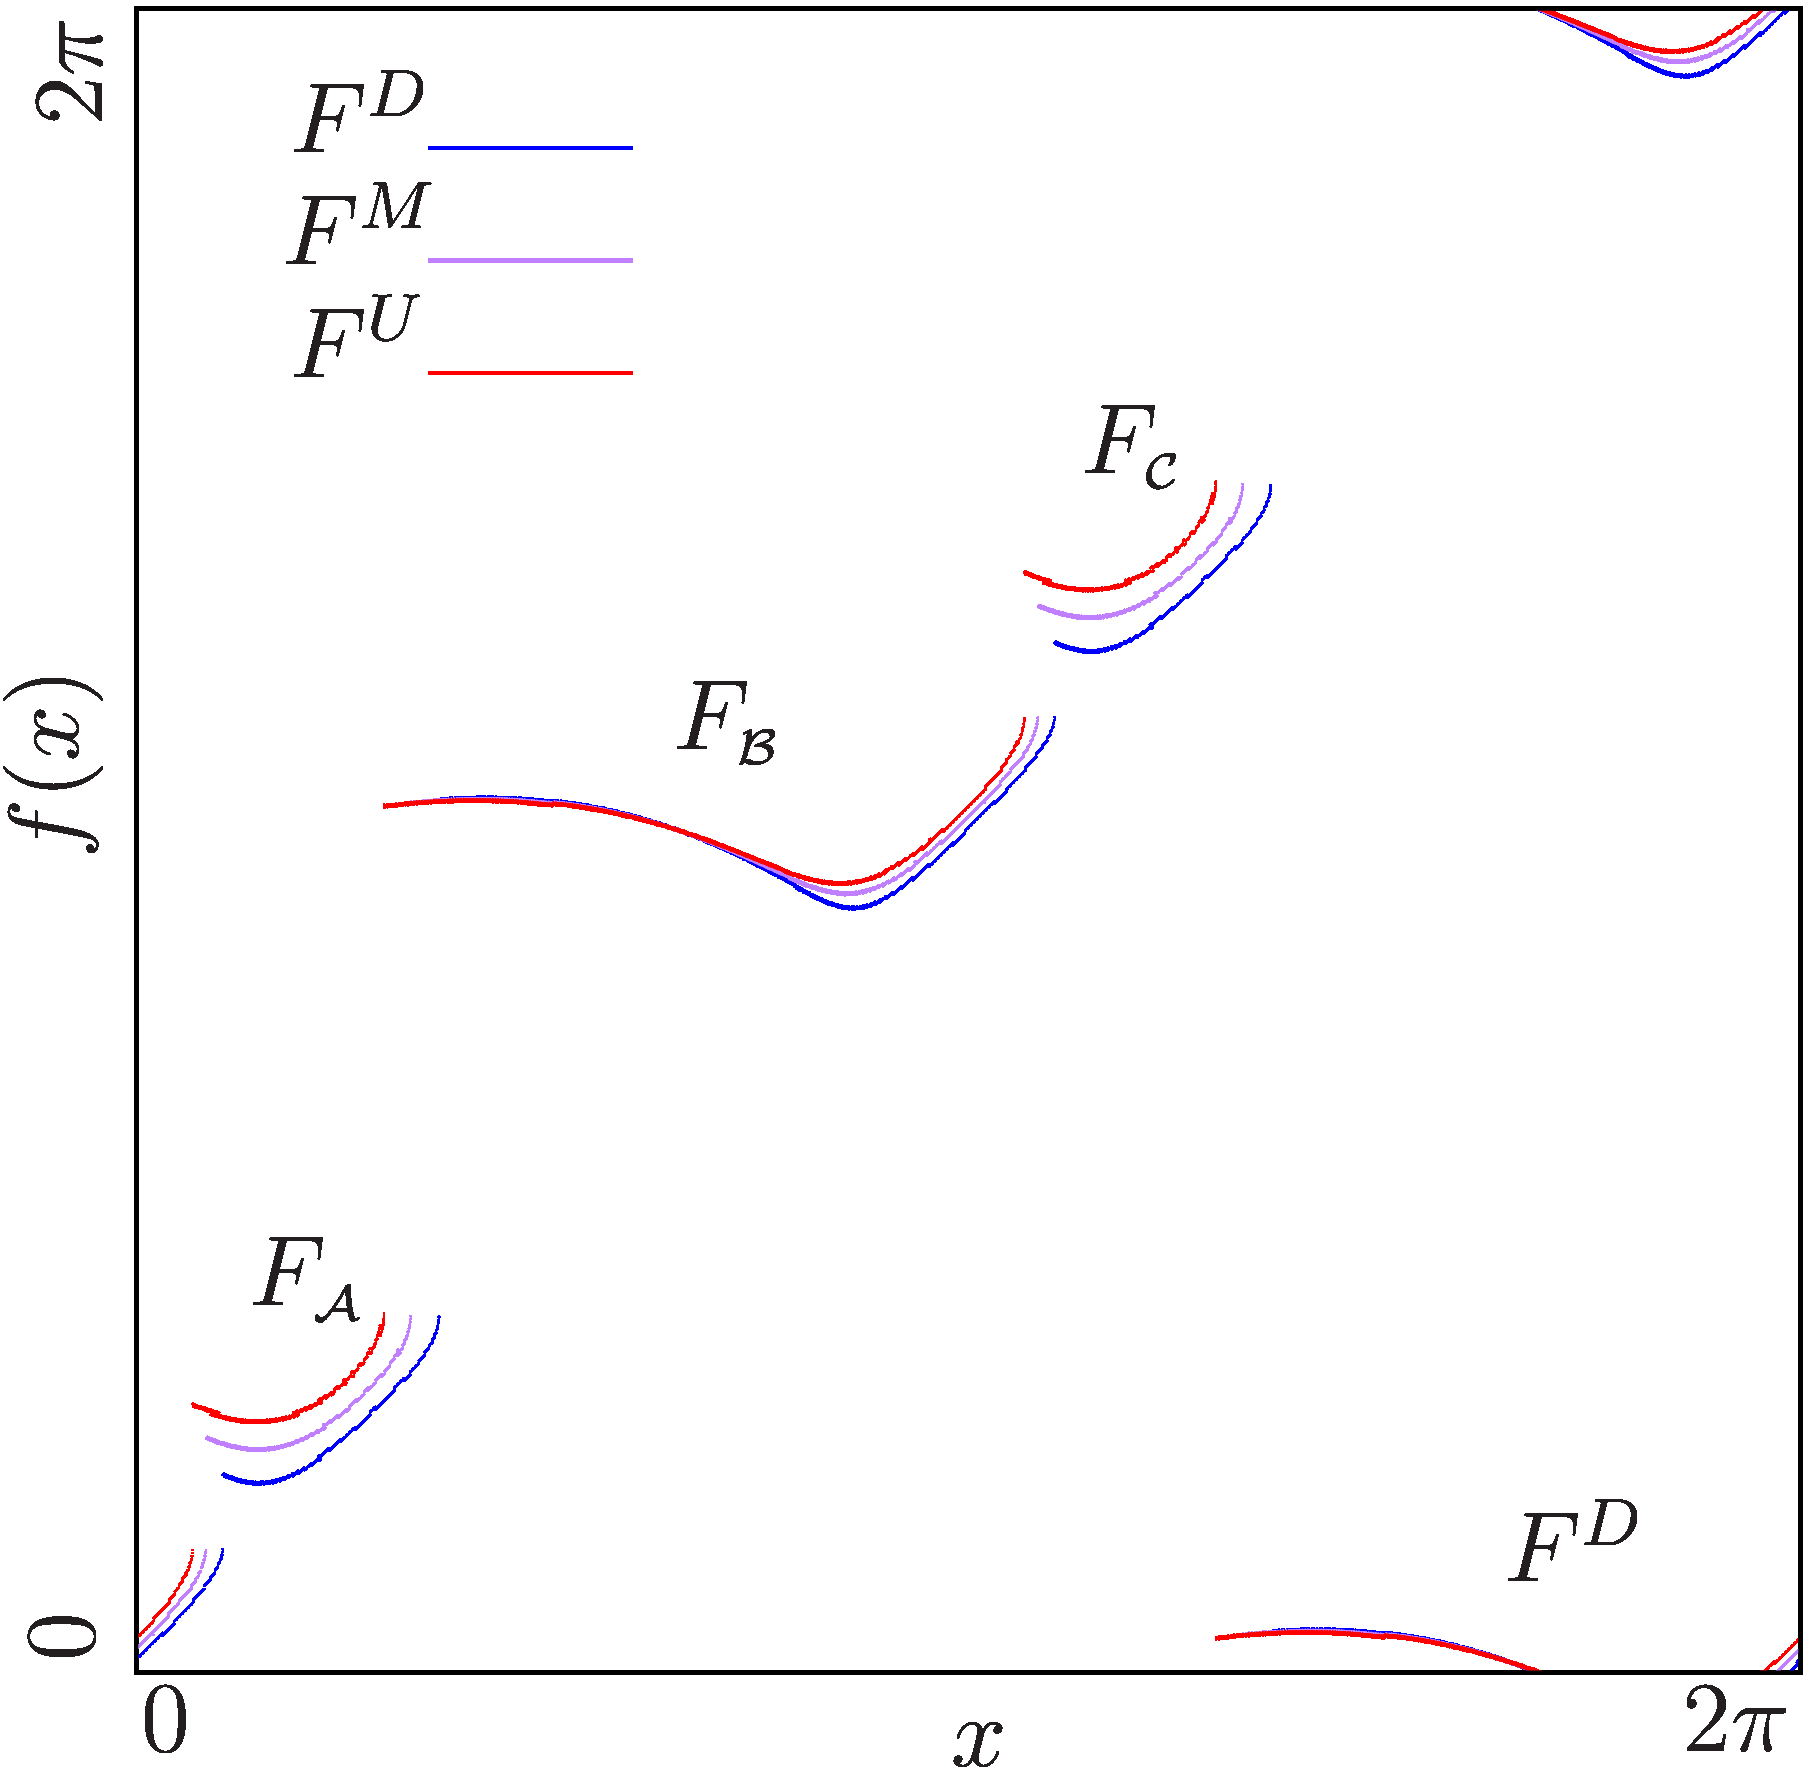
\includegraphics[width=.4 \textwidth]{../Figures/5/5.4b/illustration.png}
		\label{fig:setup.char.evolution.hi}
	}
	\caption[The isolated effects of the parameters on the original model function]{
		The isolated effects of the parameters $E_0$ and $\chi_0$ on the original model function.
		The parameter values used for plotting the functions are marked with points in \Cref{fig:setup.char.evolution.single.map}.
		(a) shows the evolution of the shape of the model function for different parameter values of $E_0$ while $\chi_0 = 0.2$ is fixed.
		The function $F^L$ is the model function with the parameter values at the point $L$ where $E_0 = 15$,
		$F^M$ is at the point $M$ where $E_0 = 17$,
		and $F^R$ is at the point $R$ where $E_0 = 19$.
		(b) shows the evolution of the shape of the model function for different parameter values of $\chi_0$ while $E_0 = 17$ is fixed.
		The function $F^D$ is the model function with the parameter values at the point $D$ where $\chi_0 = 0.1$,
		$F^M$ is at the point $M$ where $\chi_0 = 0.2$,
		and $F^U$ is at the point $U$ where $\chi_0 = 0.3$.
	}
	\label{fig:setup.char.evolution.single}
\end{figure}

\subsection{Decomposition of Combined Effects}
\label{sec:yunus.param.effects.decomposition}

This section considers the decomposition of the combined parameter effects listed in \Cref{sec:setup.char.paramfx.combined} into the effects of the isolated parameter effects listed in \Cref{sec:setup.char.paramfx.individual} and traces each effect back to its cause.
This is important, because some of the isolated parameter effects cancel out when the parameters are both varied as we will see later in this section.
For this, this section introduces a notation for the effects.
The effect of the values on the left side of a branch changing is denoted $\AL$, for the right side it is $\AR$, and for the whole branch it is $\AW$
The subscript indicates, which branch the change affects, and the superscript indicates, whether the values get larger $+$ or smaller $-$.
The effect of changing a local minimum is denoted as $\AMi$.
The meaning of the subscript stays the same as above, but the superscript also can include $L$ for movement to the left and $R$ for movement to the right.
Finally, the effect of moving borders is denoted as $\AB$.
The subscript now includes the two symbols of branches to which the border belongs and the superscript now has only $L$ or $R$.
For brevity, one does not write redundant branch names, so changes happening to branch $F_\A$ are also happening to branch $F_\C$.
For borders, changes to the border between branches $F_\A$ and $F_\B$ are also happening to the border between branches $F_\C$ and $F_\D$ and so on.

\Cref{table:setup.char.paramfx} lists all observed effects along the chains of parameter regions associated with cycles of the same period and their decomposition into effects of the single parameters.
The first part of the table includes all major changes observed in \Cref{sec:setup.char.paramfx.combined}.
The second part includes the minor change one can observe of the borders between the branches $f_\B$ and $f_\C$ moving to the left.
The second part also includes the changes observed in \Cref{sec:setup.char.paramfx.individual} that cancel out.
From this table we can see that $E_0$ causes the effects on the branches $F_\B$ and $F_\D$, while $\chi_0$ causes the changes to the branches $F_\A$ and $F_\C$, as well as the minor movement of the borders between the branches $F_\B$ and $F_\C$.
Note again that the change to the border of branches $F_\B$ and $F_\C$ also applies for the border between branches $F_\D$ and $F_\A$.

% table in next section for better layout


\section{Constructing Models}
\label{sec:setup.models}

Now that we have analyzed the original model function and know its characteristics, we start constructing different models with similar characteristics.
In this section, we will only highlight the models on the ``good'' path.
Other models that we also examined are listed in \Cref{chap:app.models}.

\subsection{Piecewise Quadratic Model}

We start with a model that is piecewise quadratic.
In the original model, the branches $f_\B$ and $f_\D$ are shaped more like cubic functions, but to keep the number of parameters low at the beginning, we model them as quadratic here.
The model has 4 branches and the same symmetry as the original model function.
We define the domain here as $[0, 6]$ instead of $[0, 2\pi]$.

The model is defined as the map $x_{n+1} = f(x_n) \mod 6$.
Where $f$ is given by the following collection of equations.
\begin{align}
	f(x) & = \begin{cases}
		         g(x)     & \text{if } r(x) < 3 \\
		         g(x) + 3 & \text{else}
	         \end{cases} \label{equ:quad.full.f}                                         \\
	g(x) & = \begin{cases}
		         a_L \cdot s_L(x)^2 + b_L \cdot s_L(x) + c_L & \text{if } s(x) < \frac{3}{2} \\
		         a_R \cdot s_R(x)^2 + b_R \cdot s_R(x) + c_R & \text{else}
	         \end{cases} \label{equ:quad.full.g}
\end{align}

\Cref{equ:quad.full.f} explicitly states the discontinuity at $0$ and $3$.
It also explicitly states the symmetry of the model.
Each half of the model is then governed by \Cref{equ:quad.full.g}.
Here all the 6 parameters $a_L, a_R, b_L, b_R, c_L,$ and $c_R$ act.

\Crefrange{equ:quad.full.s}{equ:quad.full.sr} provide adjusted values of x for both branches such that $s_L(x) = 0$ in the middle of the branches $f_\A$ and $f_\C$.
Analogous for $s_R$ and the branches $f_\B$ and $f_\D$.
\begin{subequations}
	\begin{align}
		s(x)   & = x \mod 3 \label{equ:quad.full.s}            \\
		s_L(x) & = s(x) - \frac{3}{4}                          \\
		s_R(x) & = s(x) - \frac{9}{4} \label{equ:quad.full.sr}
	\end{align}
\end{subequations}

\subsection{Centered Parabola-shaped Branches}
\label{sec:setup.quad.even}

\hl{This section examines the piecewise-quadratic model with the centered parabola-shaped branches, see the functions in} \Cref{fig:setup.quad.even.cobwebs}.
\hl{
	To center the parabola-shaped branches, the parameter values $a_L = a_R = 6$, $b_L = -\frac{3}{2}$, and $b_R = -\frac{9}{2}$ are chosen and only the parameters $c_L$ and $c_R$ are varied.
	Both varied parameters are in the ranges $[0.25, 0.6]$.
}


This emulates the effect that $\chi_0$ has on the branches $F_\A$ and $F_\C$.
Increasing $c_L$ increases the values of the branches $f_\A$ and $f_\C$.
\hl{
	The effects of $E_0$ on branches $F_\B$ and $F_\D$ are lowering the values of the function on the left sides of the branches, moving the local minima of the branches to the left, and reducing the value of the function at the minima.
}
Decreasing $c_R$ does not have the same effects \hl{on the branches $f_\B$ and $f_\D$} but rather lowers the \hl{values of the function for} the whole branches.
\Cref{fig:setup.quad.even.period.full} \hl{shows 2D scans of the periods associated with parameter regions in this model}.

\begin{figure}
	\centering
	\subfloat[Full]{
		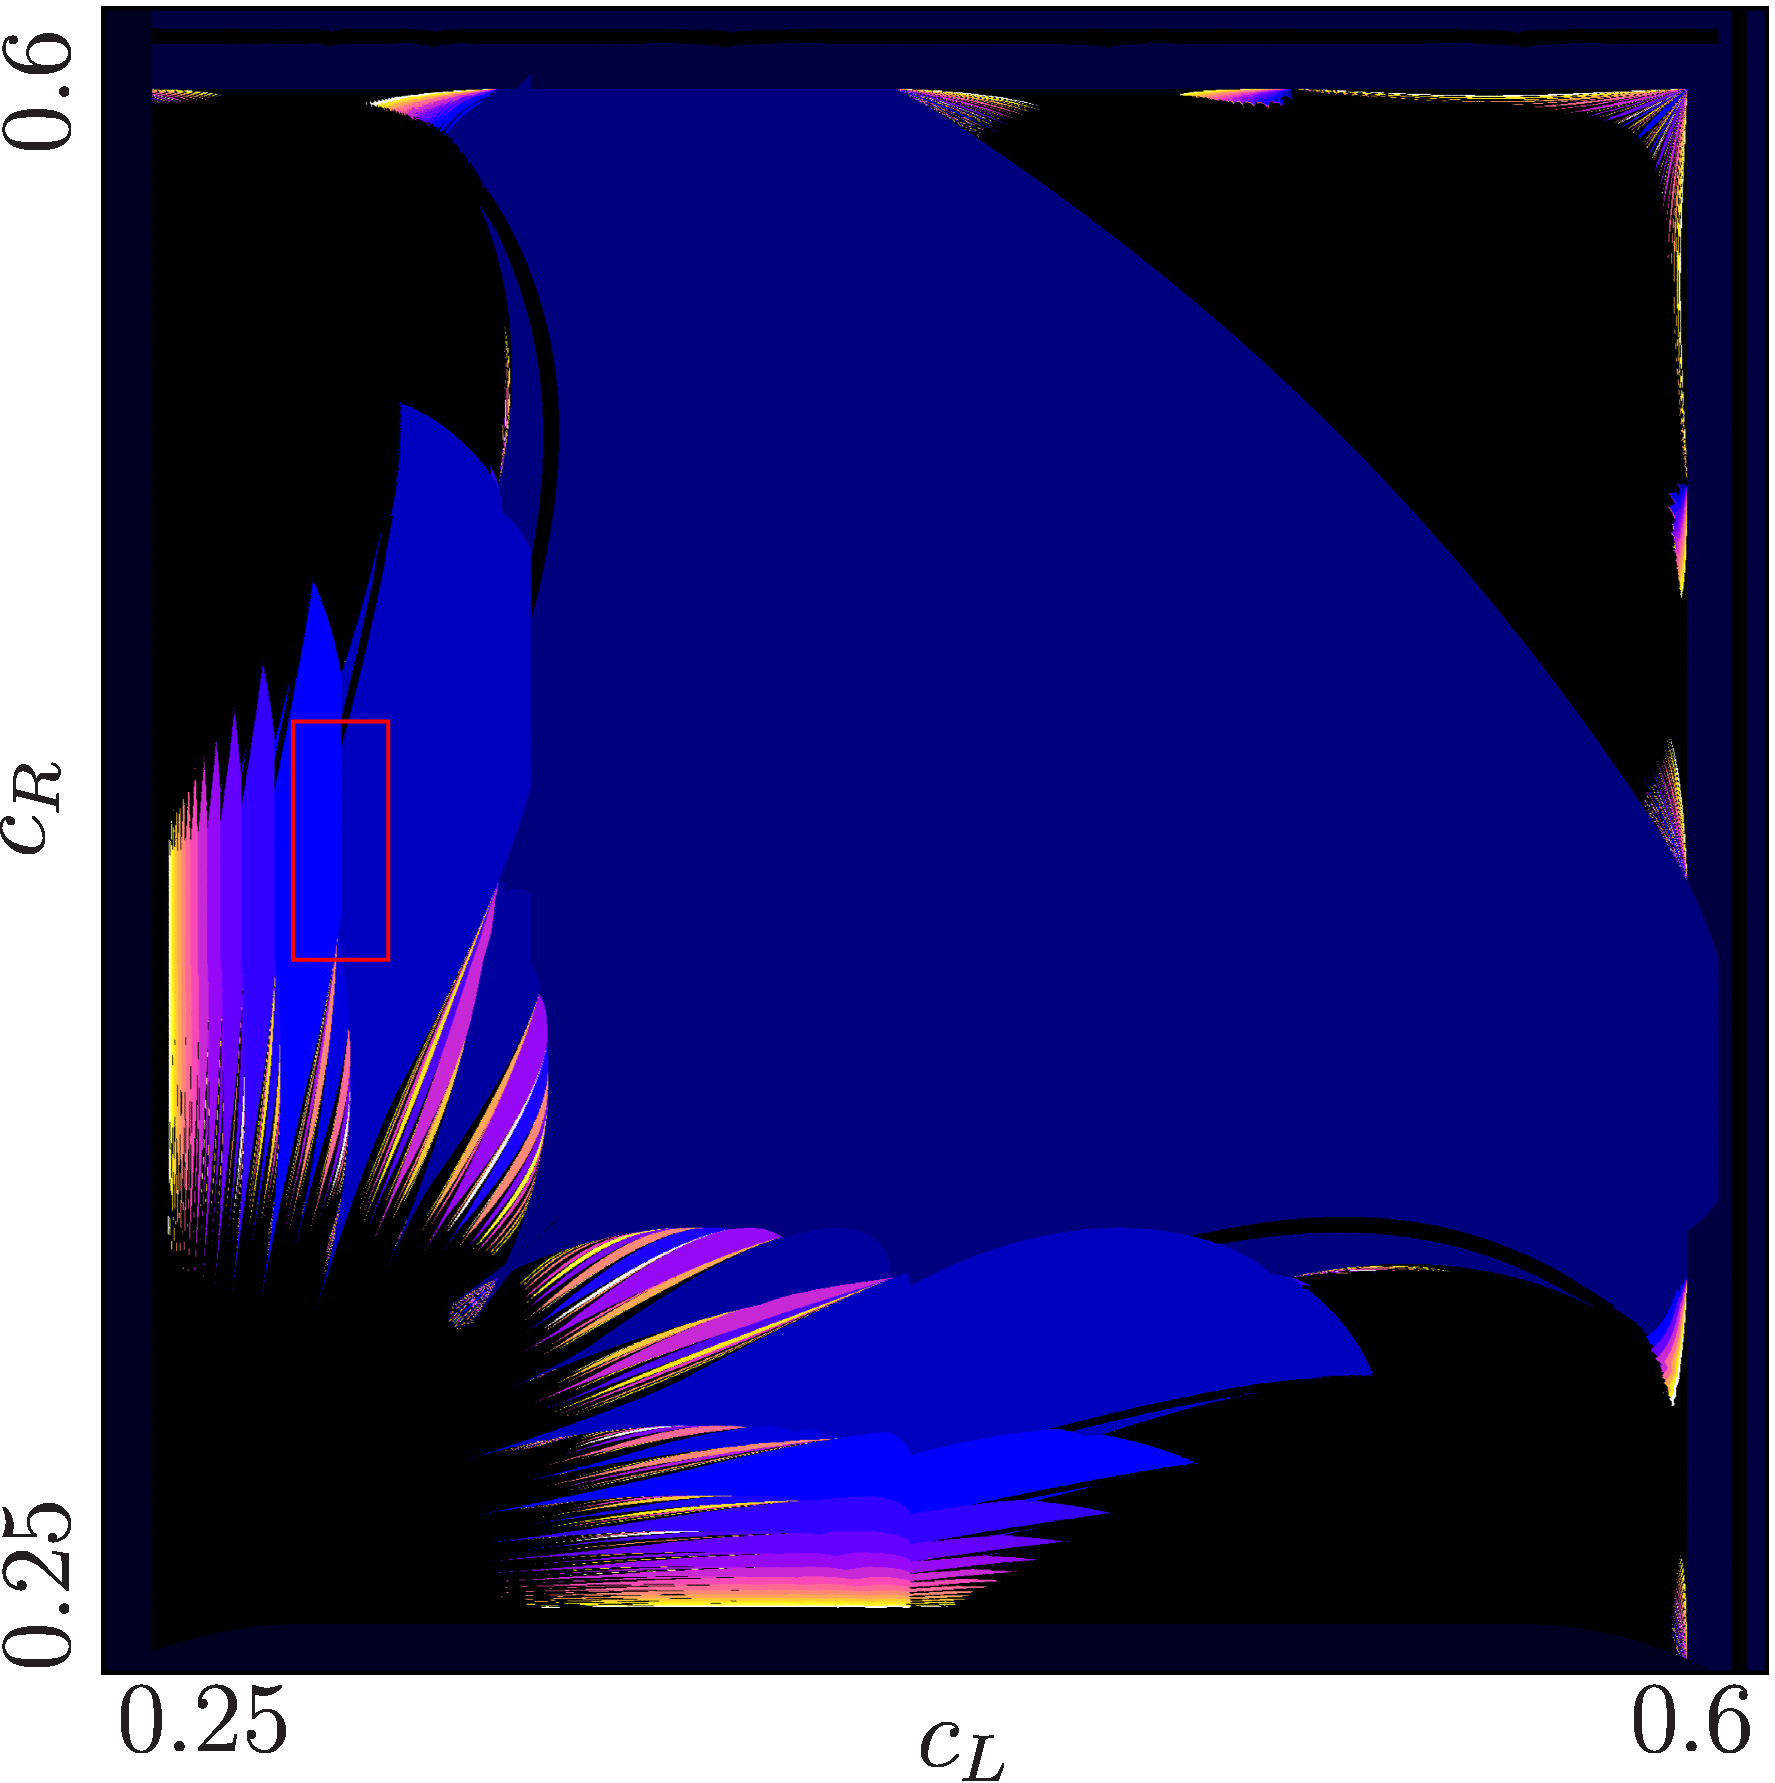
\includegraphics[width=.48 \textwidth]{../Figures/5/5.5a/result.png}
		\label{fig:setup.quad.even.period.full}
	}
	\subfloat[Zoomed]{
		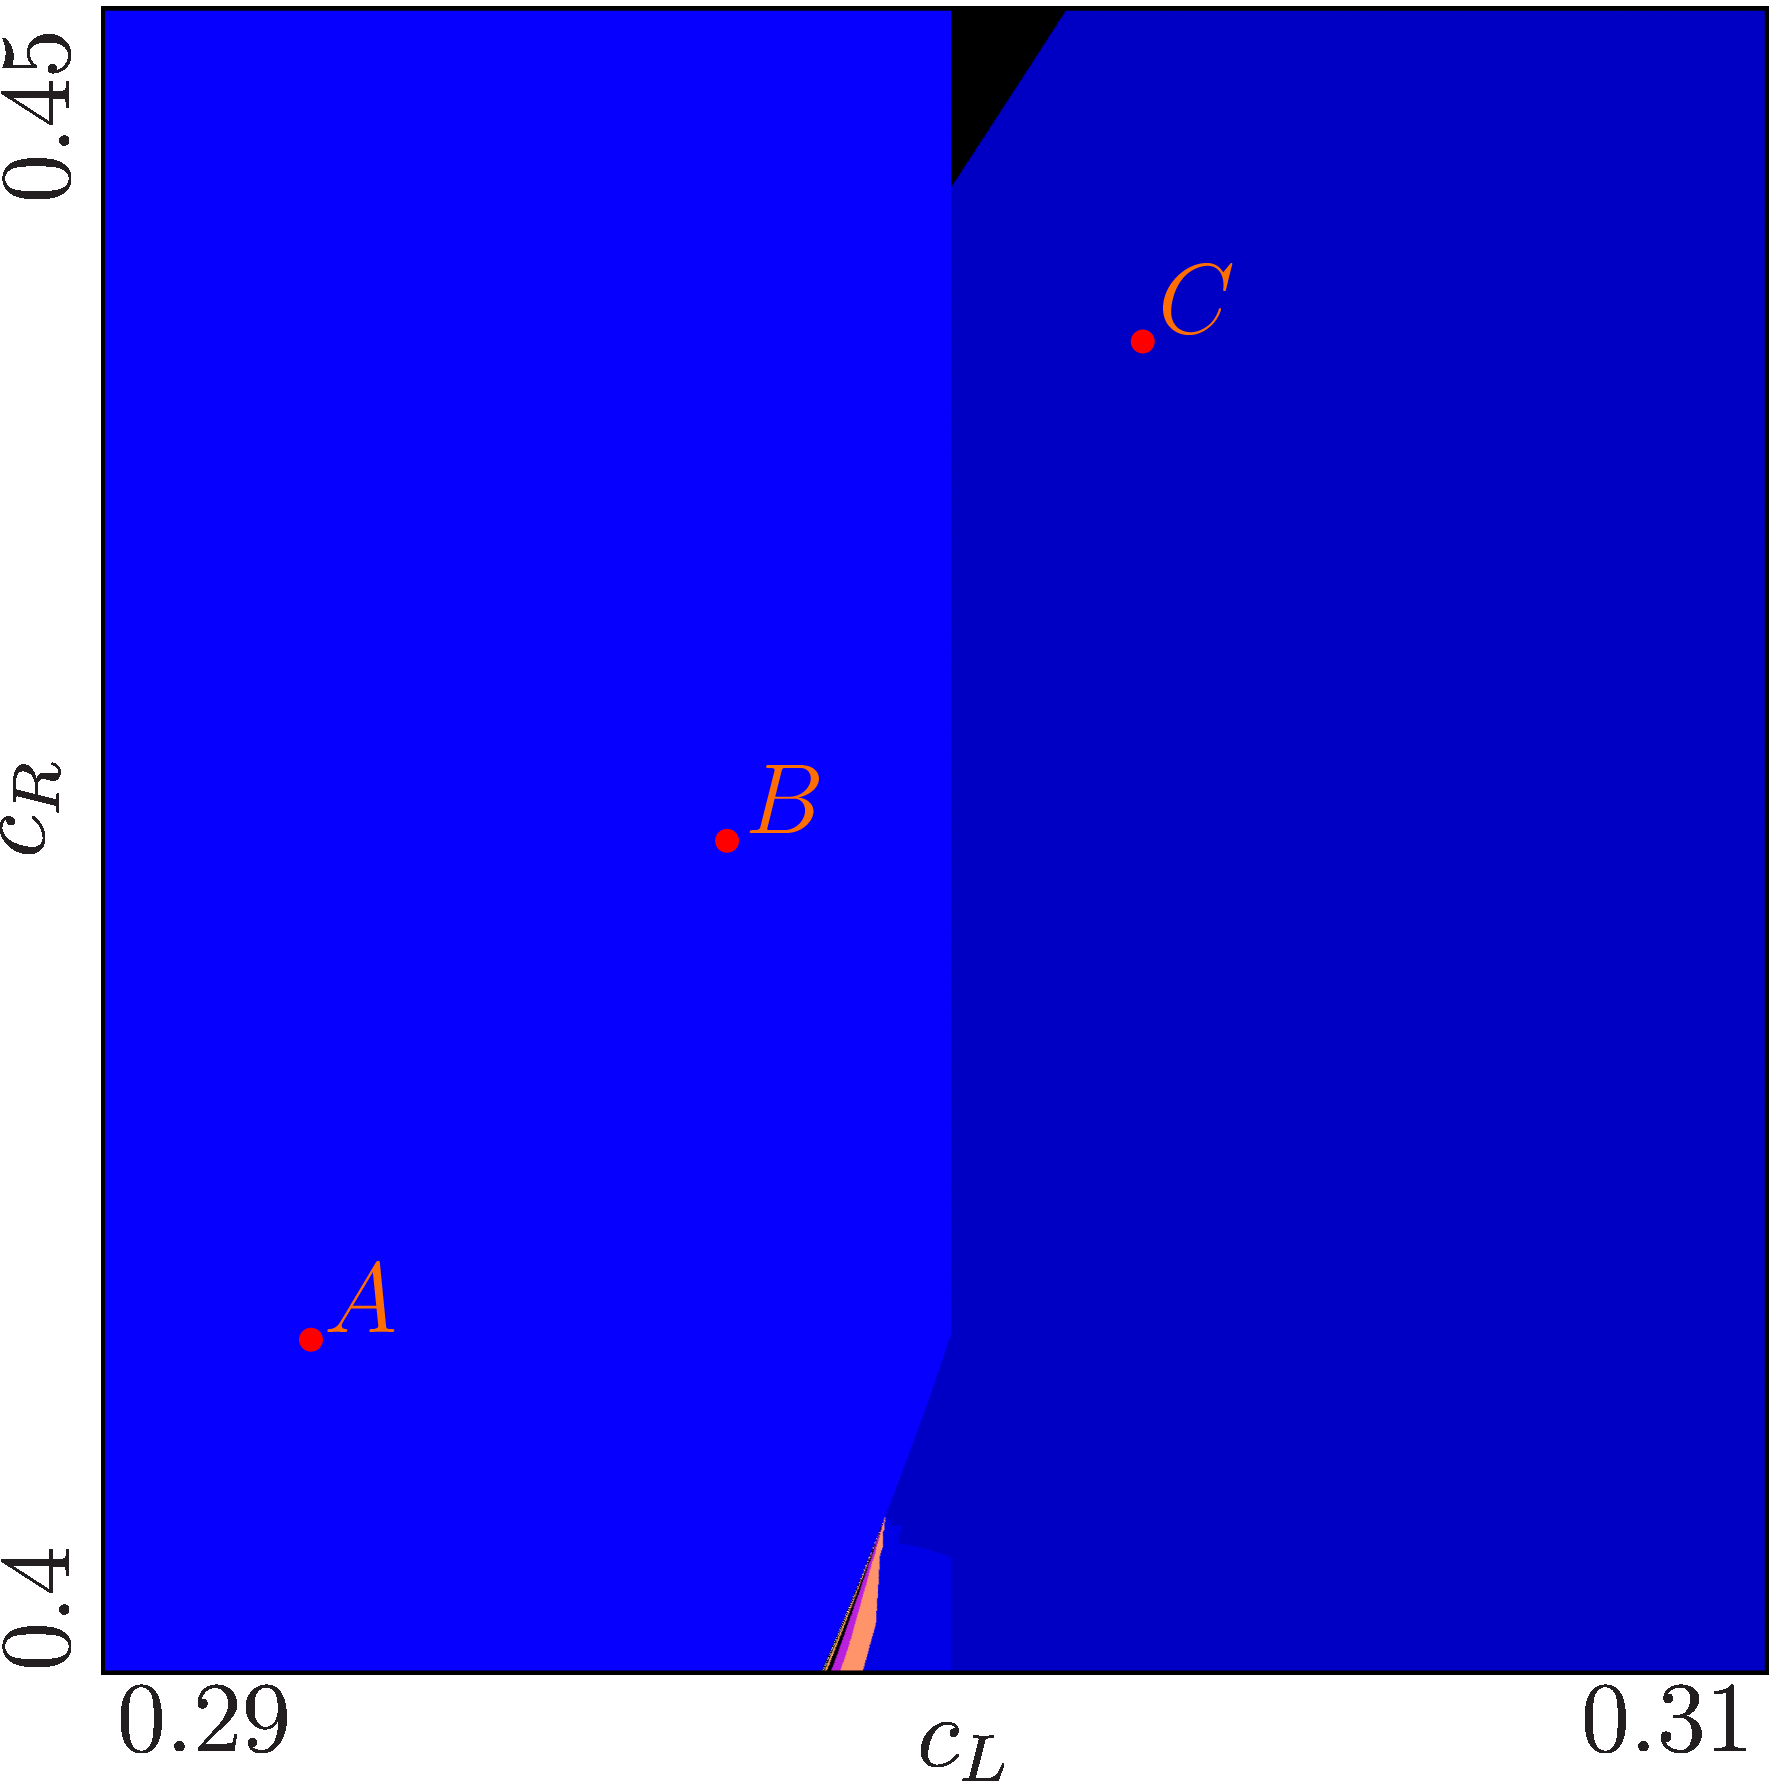
\includegraphics[width=.48 \textwidth]{../Figures/5/5.5b/result.png}
		\label{fig:setup.quad.even.period.zoomed}
	}
	\caption[2D scans showing periods of the even piecewise quadratic model]{
		2D scans showing the periods of the \hl{piecewise-quadratic} model with fixed parameters $a_L = a_R = 6$, $b_L = -\frac{3}{2}$, and $b_R = -\frac{9}{2}$.
		(a) shows the full structure with parameters $c_L$ and $c_R$ varied in the range $[0.25, 0.6]$ each.
		The red rectangle marks the parameter range that \hl{is shown magnified in} (b).
		The marked points in (b) are the parameter values for the \hl{cobweb diagrams} in \Cref{fig:setup.quad.even.cobwebs}
	}
\end{figure}

\begin{figure}
	\centering
	\subfloat[$A$]{
		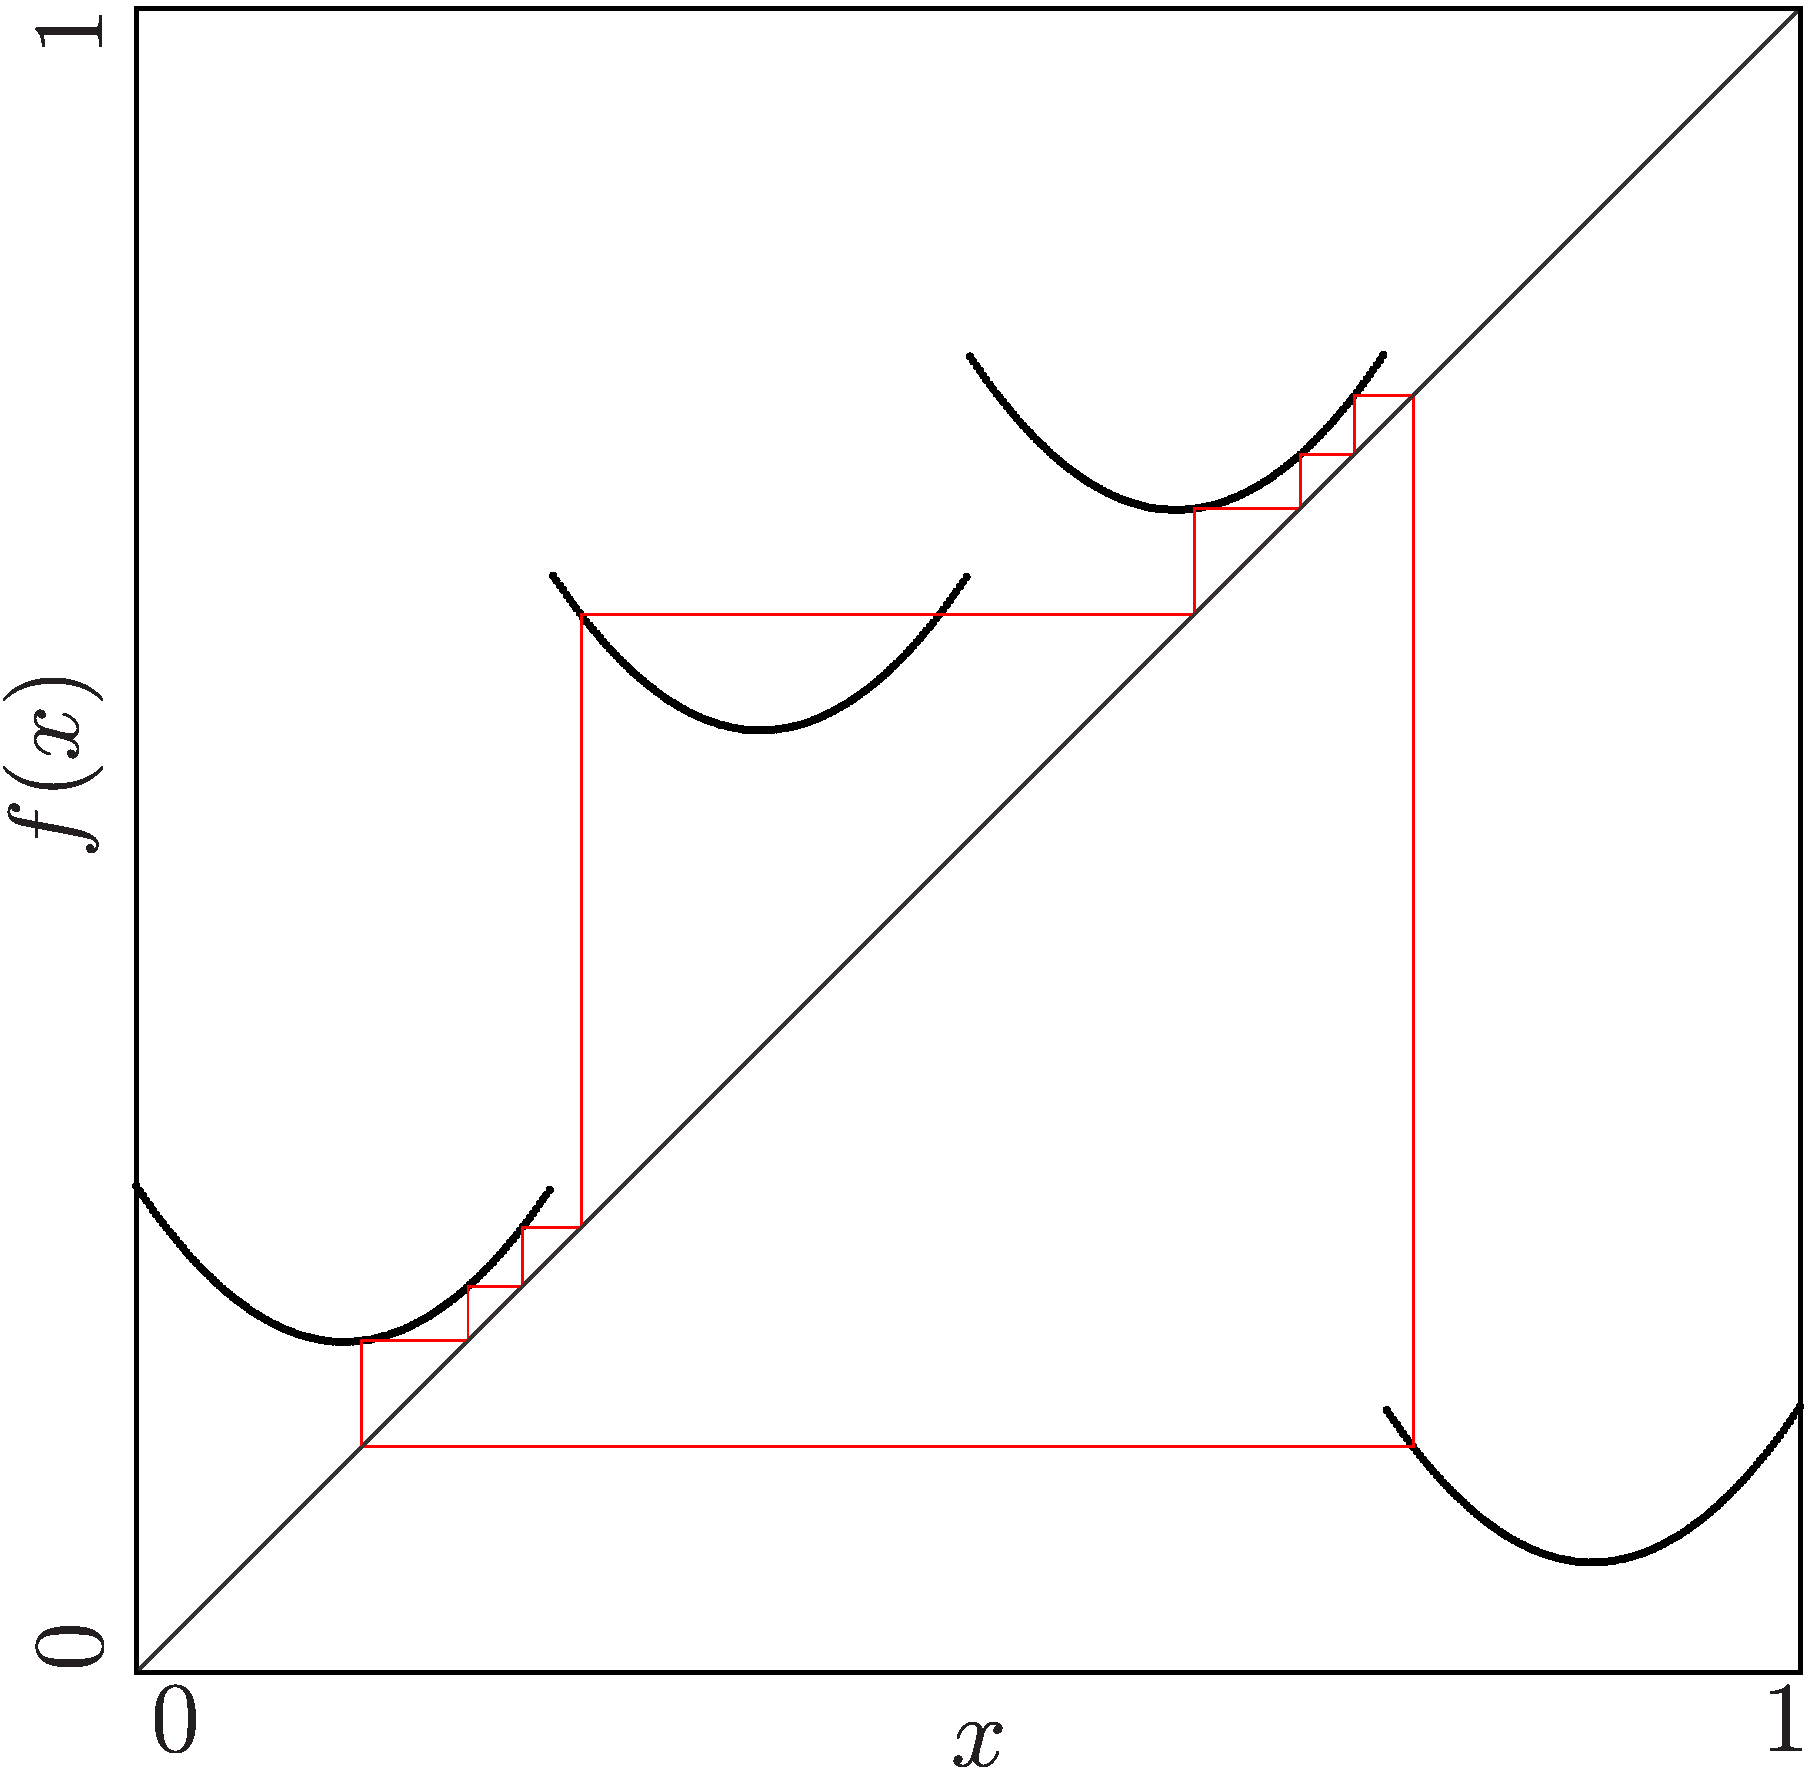
\includegraphics[width=.3 \textwidth]{../Figures/5/5.6a/result.png}
		\label{fig:setup.quad.even.cobweb.A}
	}
	\subfloat[$B$]{
		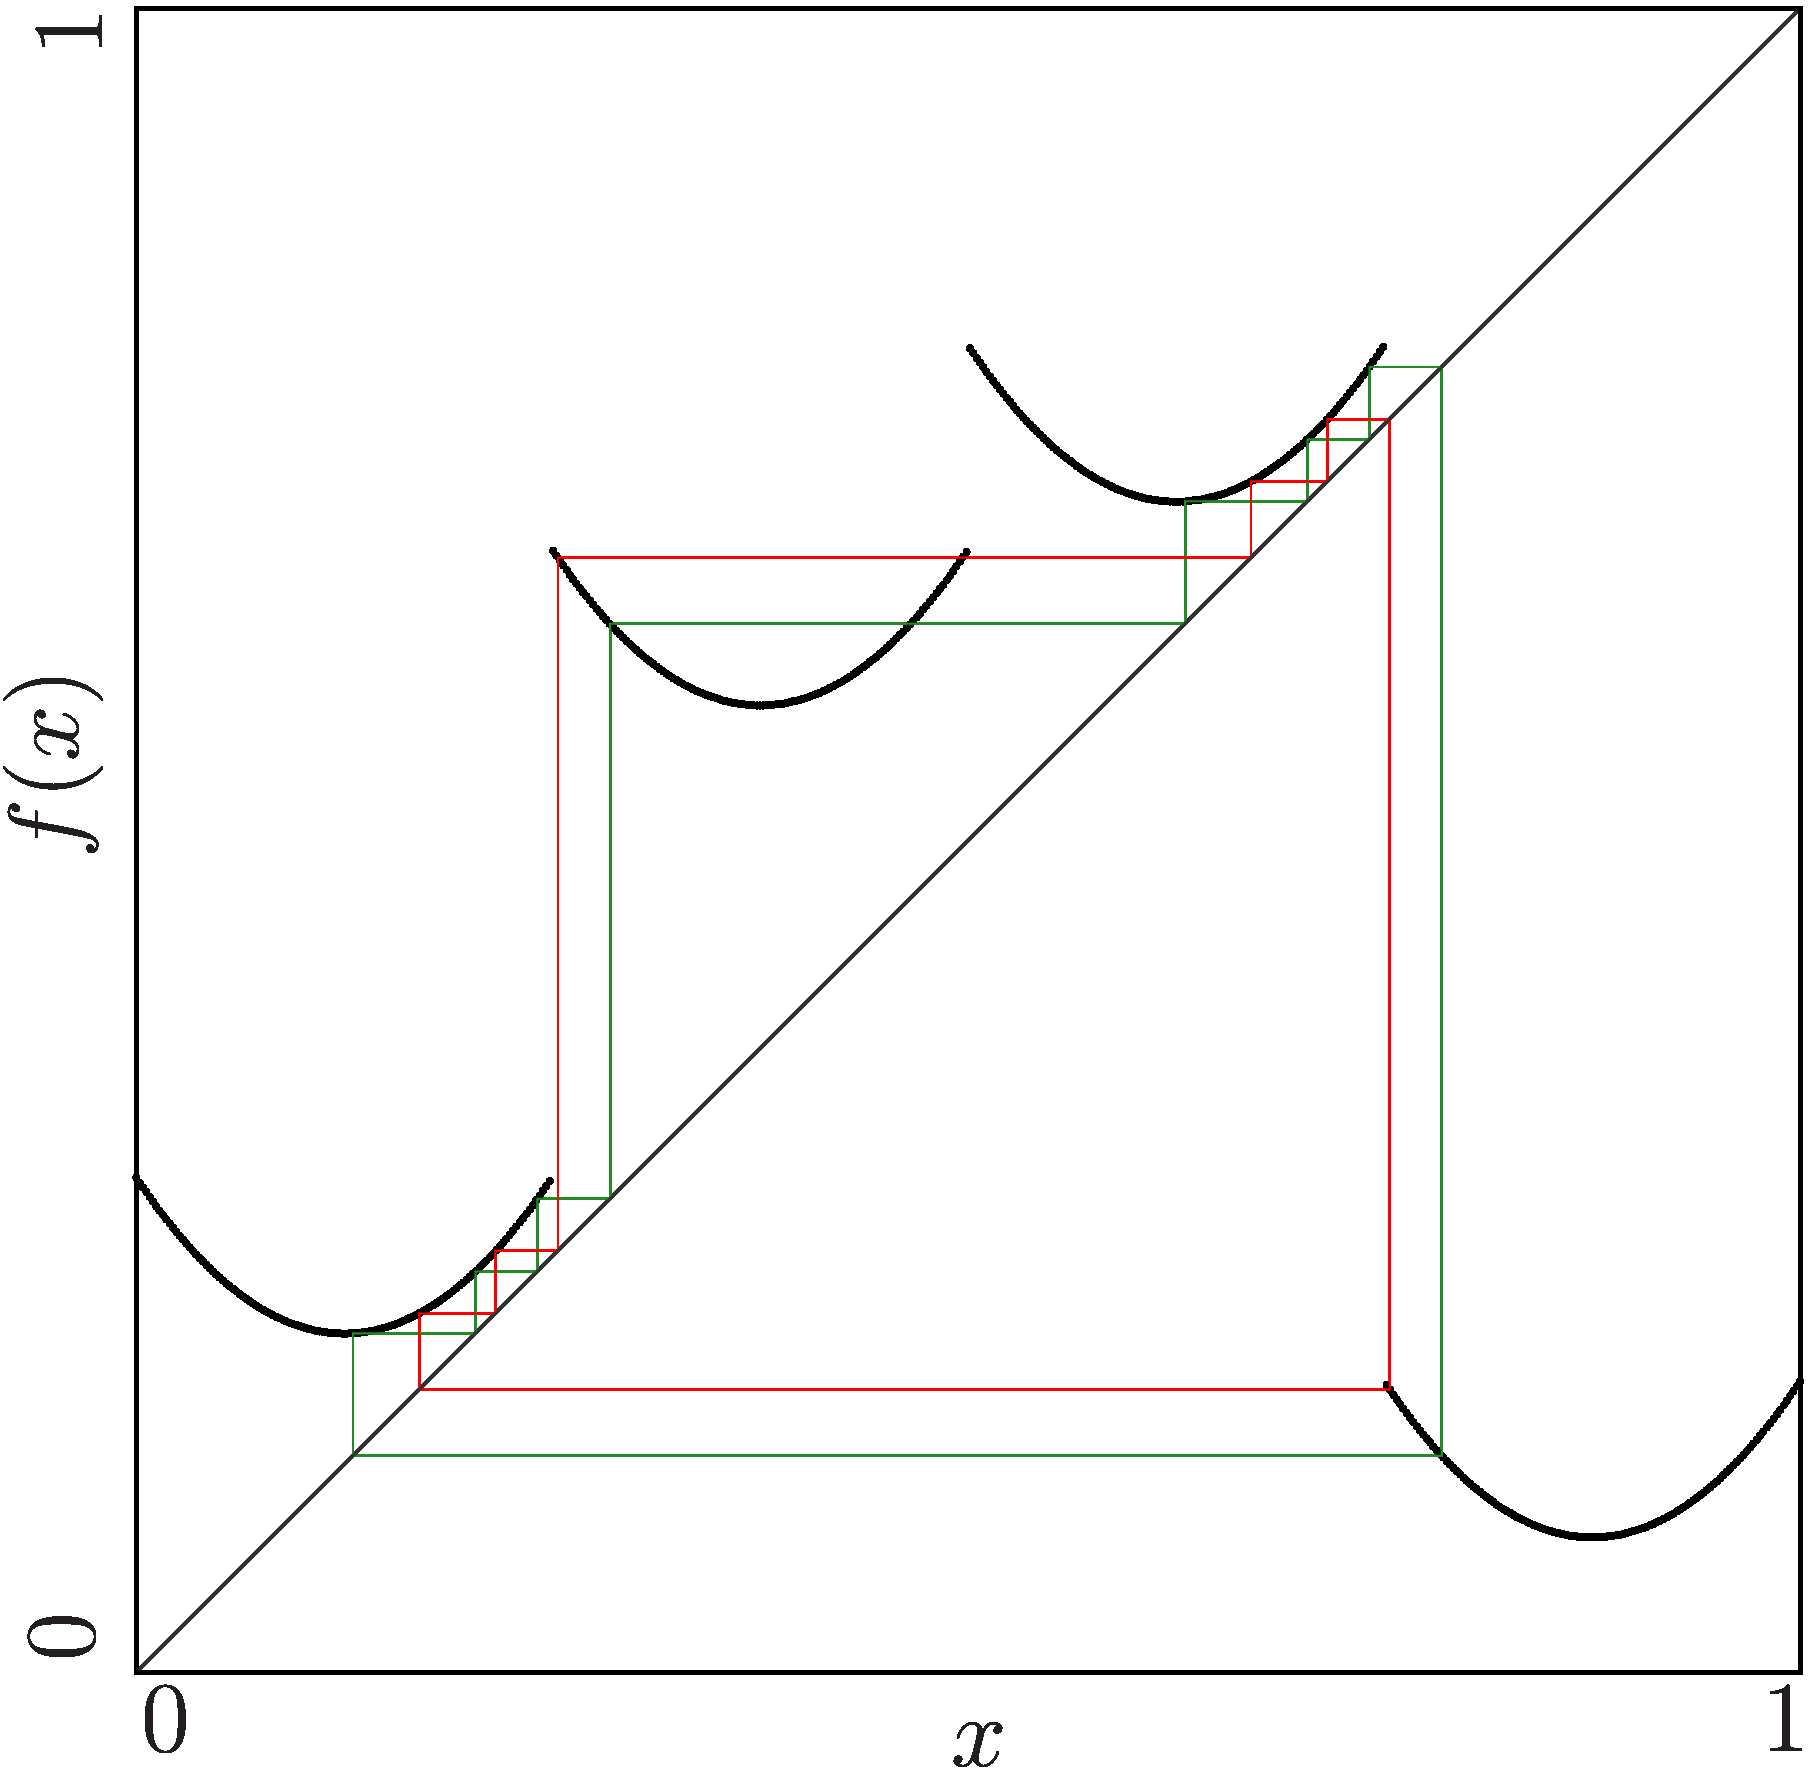
\includegraphics[width=.3 \textwidth]{../Figures/5/5.6b/result.png}
		\label{fig:setup.quad.even.cobweb.B}
	}
	\subfloat[$C$]{
		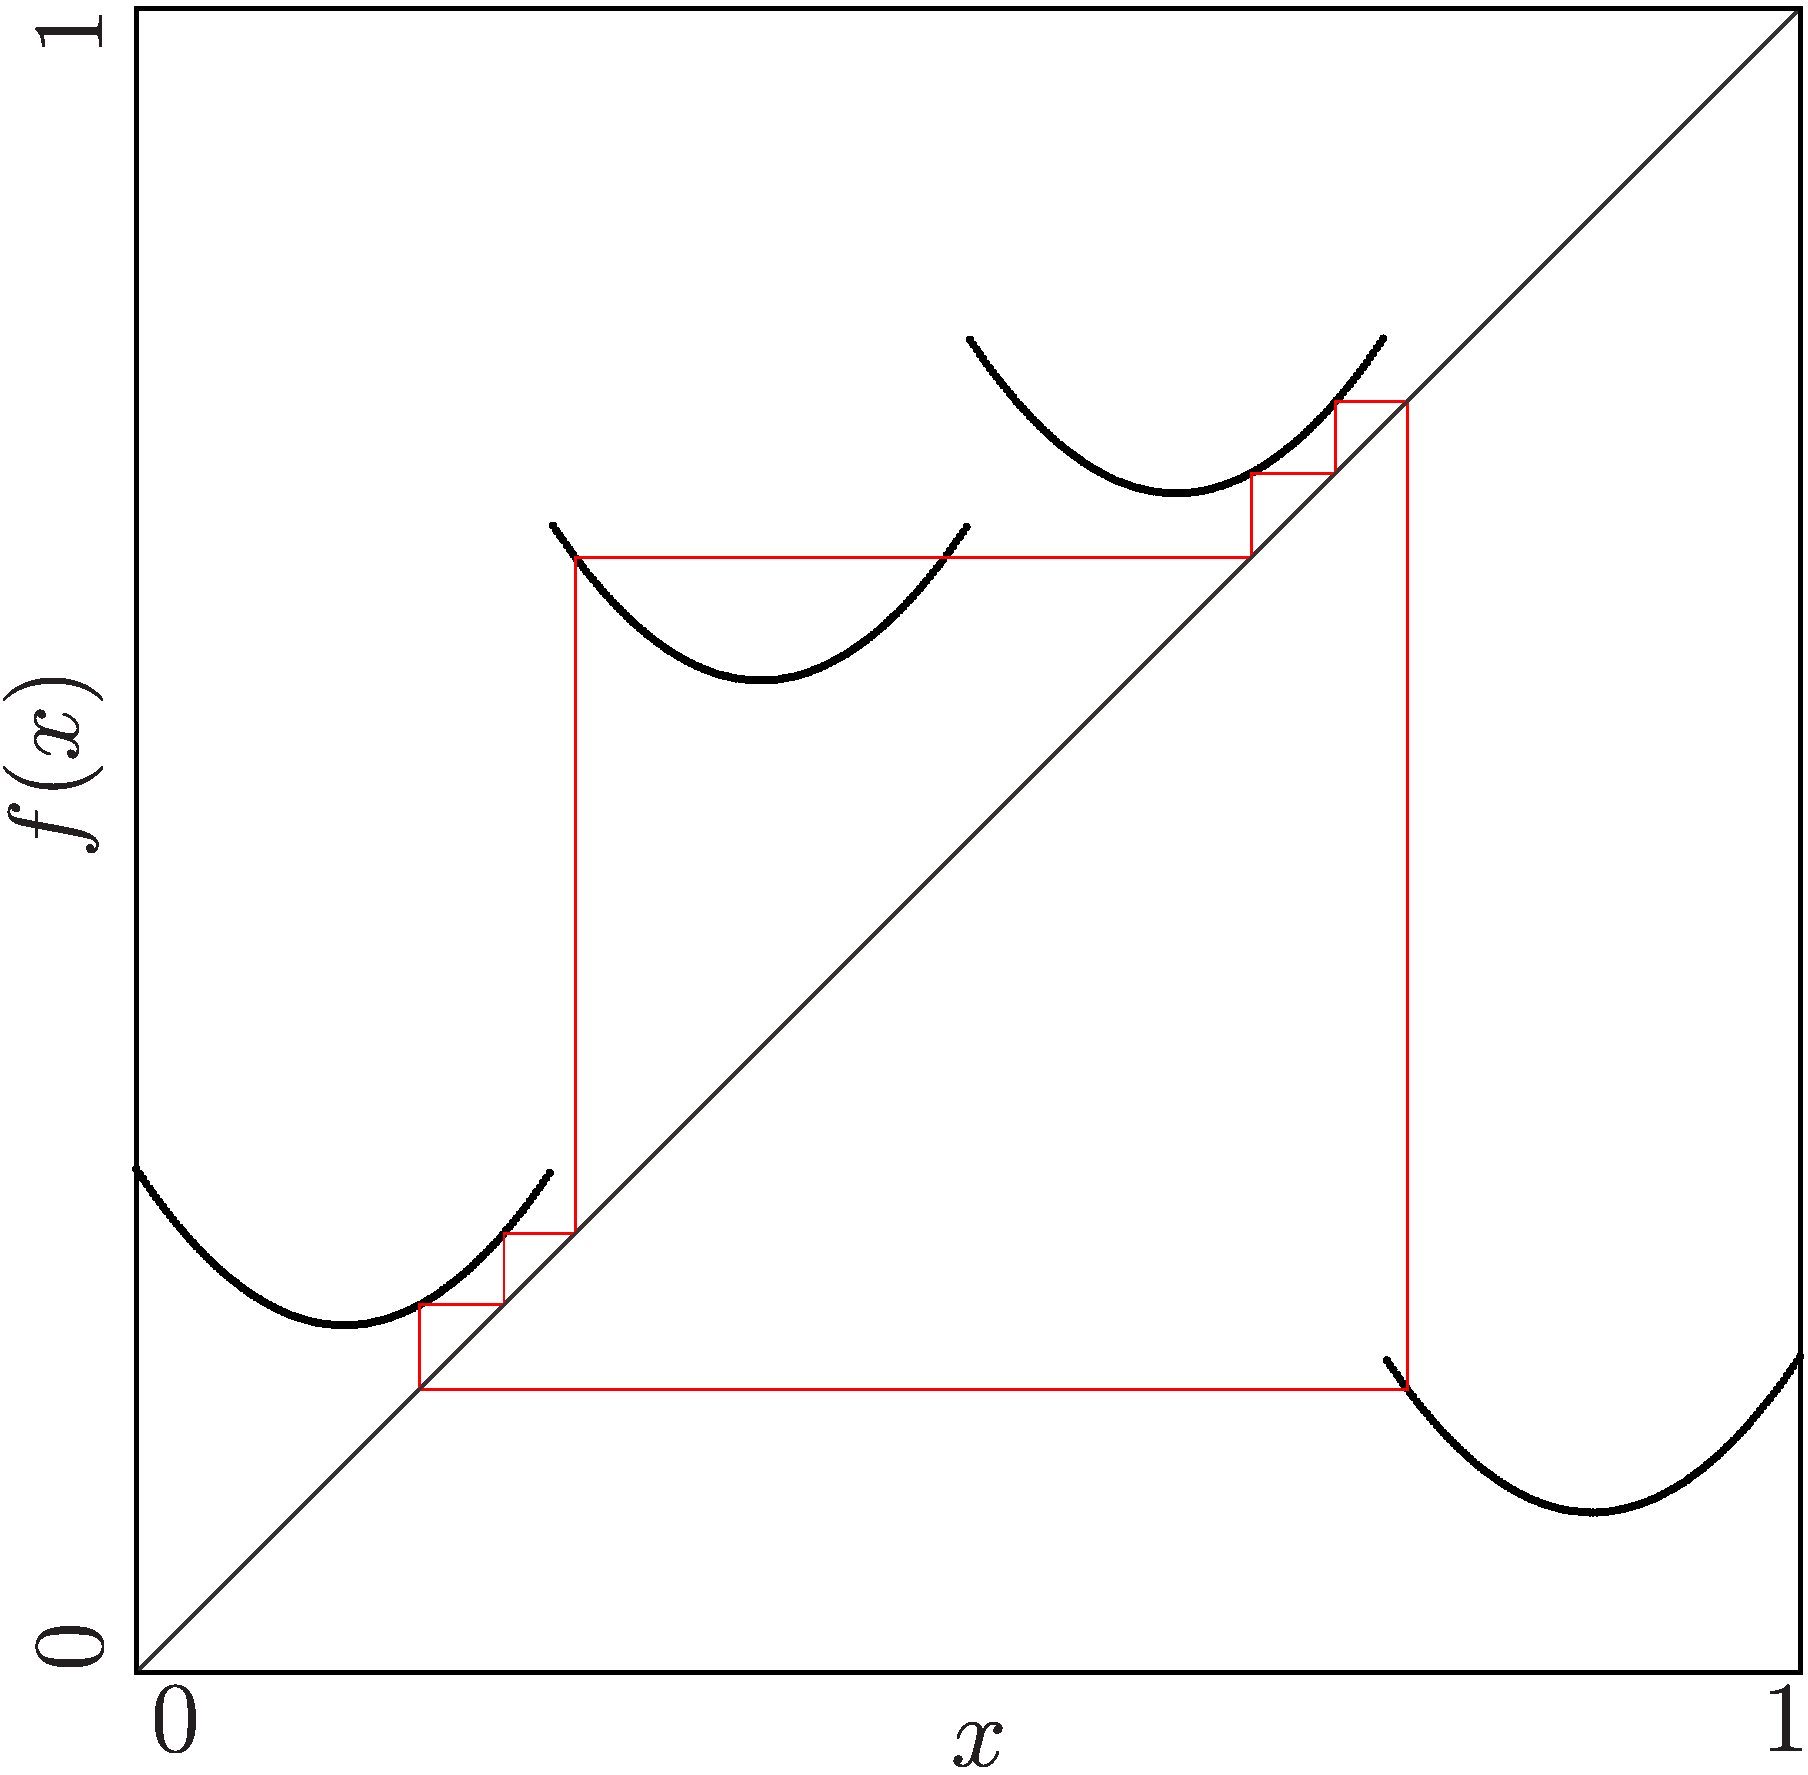
\includegraphics[width=.3 \textwidth]{../Figures/5/5.6c/result.png}
		\label{fig:setup.quad.even.cobweb.C}
	}
	\caption[Cobweb diagrams of the even quadratic model]{
		Cobweb diagrams at three parameter values of $c_L$ and $c_R$ in the piecewise quadratic model with fixed parameters $a_L = a_R = 6$, $b_L = -\frac{3}{2}$, and $b_R = -\frac{9}{2}$.
		The parameter values are marked \hl{with the points $A, B,$ and $C$} in \Cref{fig:setup.quad.even.period.zoomed}.
		(a) shows the cycle $\Cycle{\A^3\B\C^3\D}$ at \hl{the} point $A$ \hl{where $c_L = 0.2925$ and $c_R = 0.41$},
		(b) shows the two coexisting cycles $\Cycle{\A^3\B\C^3\D}$ (green) and $\Cycle{\A^2\B\C^2\D}$ (red) at the point $B$ \hl{where $c_L = 0.2975$ and $c_R = 0.425$},
		and (c) shows the cycle $\Cycle{\A^2\B\C^2\D}$ at the point $C$ where \hl{$c_L = 0.3025$ and $c_R = 0.44$}.
	}
	\label{fig:setup.quad.even.cobwebs}
\end{figure}

A phenomenon like in the original model \hl{can} not be found here.
But something very similar happens at the border of these wings.
\Cref{fig:setup.quad.even.cobwebs} shows the cobwebs at the points marked in \Cref{fig:setup.quad.even.period.zoomed}.
At point $A$, there is one stable cycle with period $8$.
This cycle is depicted in \Cref{fig:setup.quad.even.cobweb.A} and its symbolic sequence is $\A^3B\C^3\D$.
Point $B$ is in a parameter region, where 2 stable cycles coexist.
\hl{One can not} see this in the 2D scans in \Cref{fig:setup.quad.even.period.full}, since it only ever picks up on one cycle.
\Cref{fig:setup.quad.even.cobweb.B} shows the coexisting cycles at this border.
\hl{
	The symbolic sequences of the two coexisting cycles are $\A^3B\C^3\D$ and $\A^2\B\C^2\D$.
}
In contrast to the original model, the cycle that existed before in \Cref{fig:setup.quad.even.cobweb.A} \hl{with the symbolic sequence $\A^3B\C^3\D$} still exists alongside the new cycle with \hl{the symbolic sequence $\A^2\B\C^2\D$}.
\hl{
	At point $C$, there is again only one stable cycle.
	It has the period $6$ and the symbolic sequence $\A^2\B\C^2\D$.
	Therefore, this is the cycle that coexisted with the cycle with the symbolic sequence $\A^3B\C^3\D$ at point $C$.
}

This is different from the dynamics in the original model in two ways.
First, the cycles before and after the \hl{parameter region} of coexistence have different periods.
And second, the cycles existing outside the \hl{parameter region} of coexistence still exist inside the \hl{parameter region} of coexistence.
In the original model, the cycles existing outside the \hl{parameter region} of coexistence would disappear at the boundaries and new cycles would emerge inside this \hl{parameter region}.
Here, \hl{one} simply observes two overlapping parameter regions which is something different from the original model.

\subsubsection{Varying $c_L$ and $c_R$ while fixing $a_L = a_R = 6$, $b_L = -\frac{1}{2}$, and $b_R = -\frac{7}{2}$}

Choosing to make the parabolas centered was not ideal.
When looking at the original model function, one can see that the parabolas are not centered.
All branches are more skewed to the right.
To imitate this shape better, we now set $b_L = -\frac{1}{2}$ and $b_R = -\frac{7}{2}$.
All other fixed parameters are the same as above.
The parameters $c_L$ and $c_R$ are varied in the intervals $[0.08, 0.525]$ and $[0.825, 1.275]$, respectively, to capture a full structure.
\Cref{fig:setup.quad.even.period.full} shows a 2D scan of the periods of the stable cycles in this parameter range.
The structure seen in this figure repeats in all directions.

An interesting parameter area is marked with a red rectangle.
In this parameter area, 2 wings with the same period connect.
\Cref{fig:setup.quad.skew.period.zoomed} shows the 2D scan of the periods for this parameter range.
The points indicate the parameter values for the cobweb analysis.

\begin{figure}
	\centering
	\begin{subfigure}{0.4\textwidth}
		\centering
		\includegraphics[width=\textwidth]{21_Quadratic_mod1/Skew/S_2D_Period_Zoomed1/result.png}
		\caption{Full}
		\label{fig:setup.quad.skew.period.full}
	\end{subfigure}
	\begin{subfigure}{0.4\textwidth}
		\includegraphics[width=\textwidth]{21_Quadratic_mod1/Skew/S_2D_Period_Zoomed2/result.png}
		\caption{Zoomed}
		\label{fig:setup.quad.skew.period.zoomed}
	\end{subfigure}
	\caption[2D scans showing periods of the skewed piecewise quadratic model]{
		2D scans showing the periods of the piecewise quadratic model with fixed parameters $a_L = a_R = 6$, $b_L = -\frac{1}{2}$, and $b_R = -\frac{7}{2}$.
		(a) Shows the full structure with parameters $c_L$ and $c_R$ being varied in the ranges $[0.08, 0.525]$ and $[0.825, 1.275]$, respectively.
		The red rectangle marks the parameter range of (b).
		The marked points in (b) are the parameter values for the cobwebs in \Cref{fig:setup.quad.skew.cobwebs}
	}
	\label{fig:setup.quad.skew.period}
\end{figure}

\begin{figure}
	\centering
	\begin{subfigure}{0.3\textwidth}
		\centering
		\includegraphics[width=\textwidth]{21_Quadratic_mod1/Skew/S_Cobweb_A/result.png}
		\caption{At point $A$}
		\label{fig:setup.quad.skew.cobweb.A}
	\end{subfigure}
	\begin{subfigure}{0.3\textwidth}
		\centering
		\includegraphics[width=\textwidth]{21_Quadratic_mod1/Skew/S_Cobweb_B/result.png}
		\caption{At point $B$}
		\label{fig:setup.quad.skew.cobweb.B}
	\end{subfigure}
	\begin{subfigure}{0.3\textwidth}
		\centering
		\includegraphics[width=\textwidth]{21_Quadratic_mod1/Skew/S_Cobweb_C/result.png}
		\caption{At point $C$}
		\label{fig:setup.quad.skew.cobweb.C}
	\end{subfigure}
	\caption[Cobwebs of the skewed piecewise quadratic model]{
		Cobweb diagrams at three parameter values of $c_L$ and $c_R$ in the piecewise quadratic model with fixed parameters $a_L = a_R = 6$, $b_L = -\frac{1}{2}$, and $b_R = -\frac{7}{2}$.
		The parameter values are marked in \Cref{fig:setup.quad.even.period.zoomed}.
	}
	\label{fig:setup.quad.skew.cobwebs}
\end{figure}

\Cref{fig:setup.quad.skew.cobwebs} shows all the cobwebs taken at the points marked in \Cref{fig:setup.quad.skew.period.zoomed}.
The cobweb at point $A$ is shown in \Cref{fig:setup.quad.skew.cobweb.A}.
We can see that it has period 12 and its symbolic sequence is $\A^4\B^2\C^4\D^2$.
The cycle at point $C$ also has period 12.
Its cobweb diagram is shown in \Cref{fig:setup.quad.skew.cobweb.C}, and we can see that its symbolic sequence is $\A^3\B^3\C^3\D^3$.

From point $A$ to point $C$, one point of the cycle on the branch $f_\A$ moved to the branch $f_\B$.
The same thing happened to a point of the cycle on the branch $f_\C$, it moved to the branch $f_\D$.
This is similar to what happens in the original model along a chain of parameter regions with the same period.
And in between both points, there is a parameter region where 2 cycles coexist.
This is shown in \Cref{fig:setup.quad.skew.cobweb.B}, which depicts the cycles at point $C$.
But unfortunately, the coexisting cycles are the same cycles that exist at point $A$ and point $C$, $\Cycle{\A^4\B^2\C^4\D^2}$ and $\Cycle{\A^3\B^3\C^3\D^3}$.
Similarly to the previous attempt, we merely observe two parameter regions with stable cycles overlapping.

\subsubsection{Varying $c_L, a_R, b_R,$ and $c_R$ and fixing $a_L = b_L = 1$}

Now we will attempt to imitate the effects of the parameter $E_0$ on the branches $f_\B$ and $f_\D$ better.
Previously, we just varied $c_R$ which changes the values of the whole branches evenly.
Now, we only want to affect the value at the left borders of these branches.
For this, we introduce new parameters that are tied directly to characteristics of the model function.
To make this process easier, we scaled the model to the domain $[0, 4]$.
The adjusted model is $x_{n+1} = f(x_n) \mod 4$ with $f$ being defined by the following set of equations.
It is similar to the previous definition with the constant values adjusted.

\begin{align}
	f(x) & = \begin{cases}
		         g(x)     & \text{if } r(x) < 2 \\
		         g(x) + 2 & \text{else}
	         \end{cases}                                             \\
	g(x) & = \begin{cases}
		         g_L(x) = a_L \cdot s_L(x)^2 + b_L \cdot s_L(x) + c_L & \text{if } s(x) < 1 \\
		         g_R(x) = a_R \cdot s_R(x)^2 + b_R \cdot s_R(x) + c_R & \text{else}
	         \end{cases}
\end{align}
\begin{subequations}
	\begin{align}
		s(x)   & = x \mod 2           \\
		s_L(x) & = s(x) - \frac{1}{2} \\
		s_R(x) & = s(x) - \frac{3}{2}
	\end{align}
\end{subequations}

The new parameters are $g_R(1)$ for the value at the left border of branches $f_\B$ and $f_\D$, $g_R(2)$ for the value at the right border of the branches, and finally $\frac{d}{dx} g_R(x) |_{x = 2}$ for the slope of the branches at the right border.
We fix the parameter $\frac{d}{dx} g_R(x) |_{x = 2} = 1$ to have the maximum slope being $1$.
We also fix the parameter $g_R(2) = 2 + \epsilon$ with $\epsilon = 0.1$ to have the value at the right border of the branches just above the bisector $y = x$.
The parameter left is $g_R(1)$, the value at the left border of the branches.
This parameter is varied.

\todo{Solve for parameters $a_R, b_R, c_R$}

The cobwebs show that along these regions of the same period, the symbolic sequence evolves just like the symbolic sequence evolved in the original model along the chains of the same period.
Points of the sequence jump from branches $\A$ and $\C$ to branches $\B$ and $\D$.

\todo{changing the parameters of left branch gives us gecko formation}
Lighter areas indicate the existence of ``type B'' regions.

\todo{right branch has no local minimum and steepness relatively even => replace w linear branch}

Scaling the model to the interval $[0, 1]$ and mirroring the influence of the parameter $p_x$ will give the minimal model producing the desired bifurcation structures.

\todo{how scaled}

\begin{figure}
	\centering
	\includegraphics[width=0.6\textwidth]{40_Quadratic_fittingR/2D_Period_Whole/result.png}
	\caption{2D Scan of Periods of First Fitted Quadratic Model}
	\label{fig:quadratic.full.fit.1.Period}
\end{figure}

\begin{figure}
	\centering
	\begin{subfigure}{0.3\textwidth}
		\centering
		\includegraphics[width=\textwidth]{40_Quadratic_fittingR/Cobweb_A/result.png}
		\caption{At Point A}
		\label{fig:quad.full.fit.1.CobwebA}
	\end{subfigure}
	\begin{subfigure}{0.3\textwidth}
		\centering
		\includegraphics[width=\textwidth]{40_Quadratic_fittingR/Cobweb_B/result.png}
		\caption{At Point B}
		\label{fig:quad.full.fit.1.CobwebB}
	\end{subfigure}
	\begin{subfigure}{0.3\textwidth}
		\centering
		\includegraphics[width=\textwidth]{40_Quadratic_fittingR/Cobweb_C/result.png}
		\caption{At Point C}
		\label{fig:quad.full.fit.1.CobwebC}
	\end{subfigure}
	\caption{Cobwebs at Different Points}
	\label{fig:quad.full.fit.1.Cobwebs}
\end{figure}

\begin{figure}
	\centering
	\begin{subfigure}{0.4\textwidth}
		\centering
		\includegraphics[width=\textwidth]{41_Quadratic_fittingR_Gecko/2D_Period_Whole/result.png}
		\caption{Full Model}
		\label{fig:quadratic.full.fit.2.period.full}
	\end{subfigure}
	\begin{subfigure}{0.4\textwidth}
		\centering
		\includegraphics[width=\textwidth]{41_Quadratic_fittingR_Gecko/2D_Period_Whole/result-halved.png}
		\caption{Halved Model}
		\label{fig:quadratic.full.fit.2.period.halved}
	\end{subfigure}
	\caption{2D Scans of Periods of Adjusted Model...}
\end{figure}

\begin{figure}
	\centering
	\begin{subfigure}{0.3\textwidth}
		\centering
		\includegraphics[width=\textwidth]{41_Quadratic_fittingR_Gecko/Cobweb_A/result.png}
		\caption{At Point A}
		\label{fig:quad.full.fit.2.CobwebA}
	\end{subfigure}
	\begin{subfigure}{0.3\textwidth}
		\centering
		\includegraphics[width=\textwidth]{41_Quadratic_fittingR_Gecko/Cobweb_B/result.png}
		\caption{At Point B}
		\label{fig:quad.full.fit.2.CobwebB}
	\end{subfigure}
	\begin{subfigure}{0.3\textwidth}
		\centering
		\includegraphics[width=\textwidth]{41_Quadratic_fittingR_Gecko/Cobweb_C/result.png}
		\caption{At Point C}
		\label{fig:quad.full.fit.2.CobwebC}
	\end{subfigure}
	\caption{Cobwebs at Different Points}
	\label{fig:quad.full.fit.2.Cobwebs}
\end{figure}

\begin{figure}
	\centering
	\begin{subfigure}{0.4\textwidth}
		\centering
		\includegraphics[width=\textwidth]{50_Quadratic_linearR/2D_Period_Whole/result.png}
		\caption{Full Model}
		\label{fig:quadratic.full.fit.lin.period.full}
	\end{subfigure}
	\begin{subfigure}{0.4\textwidth}
		\centering
		\includegraphics[width=\textwidth]{50_Quadratic_linearR/2D_Period_Whole/result-halved.png}
		\caption{Halved Model}
		\label{fig:quadratic.full.fit.lin.period.halved}
	\end{subfigure}
	\caption{2D Scans of Periods of Adjusted Model...}
\end{figure}

\begin{figure}
	\centering
	\begin{subfigure}{0.3\textwidth}
		\centering
		\includegraphics[width=\textwidth]{50_Quadratic_linearR/Cobweb_A/result.png}
		\caption{At Point A}
		\label{fig:quad.full.fit.lin.CobwebA}
	\end{subfigure}
	\begin{subfigure}{0.3\textwidth}
		\centering
		\includegraphics[width=\textwidth]{50_Quadratic_linearR/Cobweb_B/result.png}
		\caption{At Point B}
		\label{fig:quad.full.fit.lin.CobwebB}
	\end{subfigure}
	\begin{subfigure}{0.3\textwidth}
		\centering
		\includegraphics[width=\textwidth]{50_Quadratic_linearR/Cobweb_C/result.png}
		\caption{At Point C}
		\label{fig:quad.full.fit.lin.CobwebC}
	\end{subfigure}
	\caption{Cobwebs at Different Points}
	\label{fig:quad.full.fit.lin.Cobwebs}
\end{figure}

\begin{figure}
	\centering
	\begin{subfigure}{0.4\textwidth}
		\centering
		\includegraphics[width=\textwidth]{99_Yunus/2D_Period_Zoomed/result.png}
		\caption{Original Model Full}
		\label{fig:quad.final.comparison.og.full}
	\end{subfigure}
	\begin{subfigure}{0.4\textwidth}
		\centering
		\includegraphics[width=\textwidth]{52_Quadratic_linearR_scaled_mirrored/2D_Period_Whole/result.png}
		\caption{Final Model Full}
		\label{fig:quad.final.comparison.fin.full}
	\end{subfigure} \\
	\begin{subfigure}{0.4\textwidth}
		\centering
		\includegraphics[width=\textwidth]{98_Yunus_modpi/2D_Period_Zoomed/result.png}
		\caption{Original Model Halved}
		\label{fig:quad.final.comparison.og.halved}
	\end{subfigure}
	\begin{subfigure}{0.4\textwidth}
		\centering
		\includegraphics[width=\textwidth]{52_Quadratic_linearR_scaled_mirrored/2D_Period_Whole/result-halved.png}
		\caption{Final Model Halved}
		\label{fig:quad.final.comparison.fin.halved}
	\end{subfigure}
	\caption{Comparison of 2D Scans of Periods of Original and Final Model}
	\label{fig:quad.final.comparison}
\end{figure}

\subsection{Piecewise Quadratic and Linear}





\section{Archetypal Model}
\todo{Move archetypal model definition here}

\section{Piecewise Hybrid Quadratic with Hyperparameters}
\label{sec:setup.pw.hybrid.quad}

The minimal model, which shows the same bifurcation phenomenon as the original model, is fairly simple.
Now there are no implicit equations and the model can be defined by the following explicit equations.
This section defines this model in two parts.
First, it defines all the explicit equations of the model which has some internal parameters.
Then it discusses the definitions of the external parameters to achieve the desired behavior.
Furthermore, this section then will discuss the effects of the parameters on the model function and compare it to the parameter effects in the original model.

The model maps $x \mapsto f(x) \mod 1$ where \Crefrange{equ:final.def.f}{equ:final.def.r} define $f$.
\begin{align}
	f(x) & = \begin{cases}
		         g(x)                                        & \text{ if } x < \frac{1}{2} \\
		         g\left(x - \frac{1}{2}\right) + \frac{1}{2} & \text{ else}
	         \end{cases}
	\label{equ:final.def.f}
	\\
	g(x) & = \begin{cases}
		         l(x) & \text{ if } x < \frac{1}{4} \\
		         r(x) & \text{ else}
	         \end{cases}
\end{align}

For the definitions of $l$ and $r$, we center the variable to better understand the effects of the coefficients.
Branches $\Branch_\A$ and $\Branch_\C$ exist on the intervals $\BranchInterval_\A = [0, \frac{1}{4})$ and $\BranchInterval_\C = [\frac{1}{2}, \frac{3}{4})$ respectively.
Therefore, we center the variable for the polynomials of these branches by moving it $0.125$ to the left.
\Cref{equ:final.def.tl} achieves this.
Branches $\Branch_\B$ and $\Branch_\D$ exist on the intervals $\BranchInterval_\B = [\frac{1}{4}, \frac{1}{2})$ and $\BranchInterval_\D = [\frac{3}{4}, 1)$ respectively.
The offset here is $\frac{3}{8}$ by the same logic and \Cref{equ:final.def.tr} achieves this.
\begin{align}
	s(x)   & = x \mod 1                                     \\
	t_L(x) & = s(x) - \dfrac{1}{8} \label{equ:final.def.tl} \\
	t_R(x) & = s(x) - \dfrac{3}{8} \label{equ:final.def.tr}
\end{align}

The actual polynomials defining $l$ and $r$ are then given by the following equations.
\begin{align}
	l(x) & = a_L \cdot t_L(x)^2 + b_L \cdot t_L(x) + c_L \\
	r(x) & = b_R \cdot t_R(x) + c_R
	\label{equ:final.def.r}
\end{align}

\subsection{The Model Parameters}

To get this model to show the desired behavior, we only change the coefficient $c_L$ directly via the parameter $p_y$ ($c_L = p_y$).
The coefficients $a_L = 4$ and $b_L = \frac{1}{2}$ are fixed.
The coefficients $b_R$ and $c_R$ are changed indirectly by the two parameters $A$ and $B$, which define characteristics of the function $r$.
$A$ is the value of the function $r$ at the left border of branch $\Branch_\B$, so $r(\frac{1}{4}) = A$.
And $B$ is the value of the function $r$ at the right border of branch $\Branch_\B$, so $r(\frac{1}{2}) = B$.
These constraints will yield the following set of equations.
\begin{subequations}
	\begin{align}
		r\left(\frac{1}{4}\right) & = - b_R \cdot \frac{1}{8} + c_R = A
		\label{equ:final.def.param.constr.A}
		\\
		r\left(\frac{1}{2}\right) & = b_R \cdot \frac{1}{8} + c_R = B
		\label{equ:final.def.param.constr.B}
	\end{align}
\end{subequations}

Solving for $b_R$ and $c_R$ will give us explicit definitions of these two internal parameters depending on both $A$ and $B$.
Adding both \Cref{equ:final.def.param.constr.A} and \Cref{equ:final.def.param.constr.B} will yield the \Cref{equ:final.def.param.cR} for $c_R$.
\begin{align}
	2 \cdot c_R = A + B \implies c_R = \dfrac{A + B}{2}
	\label{equ:final.def.param.cR}
\end{align}

Similarly, subtracting \Cref{equ:final.def.param.constr.A} from \Cref{equ:final.def.param.constr.B} will yield the \Cref{equ:final.def.param.bR} for $b_R$.
\begin{align}
	\dfrac{b_R}{4} = B - A \implies b_R = 4 \cdot (B - A)
	\label{equ:final.def.param.bR}
\end{align}

For our purposes, we also fix the parameter $B = \frac{1}{2} + \frac{1}{40}$, so that the right border of the branches $\Branch_\B$ and $\Branch_\D$ are just above the bisector.
We only change the parameter $A$ via the parameter $p_x$, where we negate the value of $p_x$ to get a similar 2D-scan to the original function.
So $A = -p_x$.

\Cref{tab:final.def.parameters.overview} lists the values of all parameters of the model.
The first part focuses on the parameters of the function $l$, while the second part lists the parameters needed for the function $r$.

\begin{table}
	\centering
	\begin{tabular}{|c|c|}
		\hline
		Model Parameter & Value                        \\ \hline \hline
		$a_L$           & $4$                          \\ \hline
		$b_L$           & $\frac{1}{2}$                \\ \hline
		$c_L$           & $p_y$                        \\ \hline \hline
		$b_R$           & $4 \cdot (B - A)$            \\ \hline
		$c_R$           & $\frac{1}{2} \cdot (A + B)$  \\ \hline
		$A$             & $-p_x$                       \\ \hline
		$B$             & $\frac{1}{2} + \frac{1}{40}$ \\ \hline
	\end{tabular}
	\caption{Overview of Parameter Values of Final Model}
	\label{tab:final.def.parameters.overview}
\end{table}

\subsection{Parameter Effects}

The effects of the parameters on the model function are straightforward and can be read directly from the previous section.
In summary, the parameter $p_x$ changes the height of the branches $\Branch_\B$ and $\Branch_\D$ at their left border, where a lower $p_x$ means a higher value of the model function at these points.
In the previously defined notation, this is written as $\AL_{\B}^-$.
This notation is defined in \Cref{sec:yunus.param.effects}.
The parameter $p_y$ changes the offset of branches $\Branch_\A$ and $\Branch_\C$, so it moves the whole branches in contrast to $p_x$.
A higher $p_y$ means a higher offset and it is written as $\AW_{\A}^+$.


\Cref{fig:final.param.effects.px,fig:final.param.effects.py} illustrate these parameter effects.
Both figures show the model function for three parameter combinations, where either $p_x$ or $p_y$ is fixed and the other parameter is changed.
The model function is colored according to the changed parameter, blue is for the lowest value and red is for the highest value.
\Cref{fig:final.param.effects.px} illustrates the effect of $p_x$.
You can see, how the left borders of branches $\Branch_\B$ and $\Branch_\D$ are lower for higher values of $p_x$.
\Cref{fig:final.param.effects.py} illustrates the effect of $p_y$.
Here one can see, how the whole branches $\Branch_\A$ and $\Branch_\C$ move up for higher values of $p_y$.

\begin{figure}
	\centering
	\begin{subfigure}{0.4\textwidth}
		\centering
		\includegraphics[width=\textwidth]{60_MinimalRepr/ParameterEffects/p_x/illustration.png}
		\caption{$p_x$}
		\label{fig:final.param.effects.px}
	\end{subfigure}
	\begin{subfigure}{0.4\textwidth}
		\centering
		\includegraphics[width=\textwidth]{60_MinimalRepr/ParameterEffects/p_y/illustration.png}
		\caption{$p_y$}
		\label{fig:final.param.effects.py}
	\end{subfigure}
	\caption{Illustration of Parameter Effects}
\end{figure}

\Cref{tab:final.def.parameters.effects} list the effects of parameters $p_x$ and $p_y$ in a table, like also done for the original model in \Cref{sec:yunus.param.effects}.
Additionally, the parameter effects of the parameters in the original model are listed for comparison.
This gives a nice overview of which characteristics of the original model function are necessary for the observed bifurcation patterns.
Especially it shows, which parameter effects are not necessary.
For example, the effect $\AMi_{\B}^{L-}$ cannot even be fabricated in this model since branches $\Branch_\B$ and $\Branch_\D$ are linear and do not have a local minimum.
Also the effect $\AB_{\B\C}^L$, which is the movement of the borders between branches $\Branch_\B$ and $\Branch_\C$ (and $\Branch_\D$ and $\Branch_\A$ respectively), is not necessary.

\begin{table}
	\centering
	\begin{tabular}{|c||c|c||c|c|} \hline
		Combined         & $E_0$            & $\chi_0$          & $p_x$        & $p_y$          \\ \hline \hline
		$\AL_{\B}^{-}$   & $\AL_{\B}^{-}$   &                   & $\AL_{\B}^-$ &                \\ \hline
		$\AMi_{\B}^{L-}$ & $\AMi_{\B}^{L-}$ & $-\AMi_{\B}^{+}$  &              &                \\ \hline
		$\AW_{\A}^{+}$   &                  & $\AW_{\A}^{+}$    &              & $\AW_{\A}^{+}$ \\ \hline \hline
		$\AB_{\B\C}^{L}$ &                  & $\AB_{\B\C}^{L}$  &              &                \\ \hline
		                 & $\AB_{\A\B}^{R}$ & $-\AB_{\A\B}^{L}$ &              &                \\ \hline
	\end{tabular}
	\caption{Comparison of Parameter Effects}
	\label{tab:final.def.parameters.effects}
\end{table}


